\documentclass[12pt]{article}
\usepackage{graphicx}
\usepackage[utf8]{inputenc}
\usepackage{makecell}
\usepackage[margin=0.7in]{geometry}
\usepackage[T1]{fontenc}
\usepackage{mathptmx}
\usepackage[normalem]{ulem}
\usepackage{hyperref}
\usepackage{array}
\usepackage{float}
\usepackage{tikz}
\usepackage{xcolor, colortbl}
\renewcommand\theadalign{bc}
\renewcommand\theadfont{\bfseries}
\renewcommand\theadgape{\Gape[4 pt]}
\renewcommand\cellgape{\Gape[4 pt]}
\renewcommand{\arraystretch}{1.5}
\setlength{\tabcolsep}{1.5 em}
\setlength{\arrayrulewidth}{1 pt} 
\usepackage[
backend=bibtex,
style=numeric,
sorting=ynt
]{biblatex}
\addbibresource{References.bib}

%opening
\title{Software Proposal Document for \\ \vspace{0.1 cm} Mele: Real-time IoT Monitoring for Beehives and Apiaries}
\author{Adam Loay, Dalia Raafat, Khaled Yehia, Moshir Ashraf and Mounir Nader\\ \vspace{0.5 cm}
	Supervised by: Dr. Walaa Hassan and Eng. Hamsa Mahmoud} 
\date{}
\begin{document}
	\maketitle
	\begin{table}[htp]
		\centering
		\vspace{-1 cm}
		\caption{Document Version History}
		\vspace{0.25 cm}
		\begin{tabular}{|l|l|l|}
			\hline
			\thead{Proposal Version}    & \thead{Date} & \thead{Reason for Change}  \\ \hline
			1.0 & 8-September-2024   & \makecell{Proposal First version}   \\
			\hline
		\end{tabular}
		
	\end{table}
	\begin{table}[htp]
		\begin{tabular}{cc}
			\thead{GitHub:} {\href{https://github.com/Quick-AI-for-ORG/Mele-RIMBA}{\textit{https://github.com/Quick-AI-for-ORG/Mele-RIMBA}}
			}   
		\end{tabular}
	\end{table}
	
	
	\begin{abstract}
		The main idea of this project is to study the ........
		(Word Limit 150)
	\end{abstract}
	
	\section{Introduction}
	
	\subsection{Background} 
	Life on Earth faces many challenges, despite our technological advances in many different fields; many humans still live in poverty and lack access to basic human necessities like food and clean water. To make matters even worse, factors such as climate change and poor agricultural practices exacerbate food scarcity worldwide by reducing the survival rate of crops. 
	Not to mention, our precious environment is also threatened by multiple contentions that result in deforestation and loss of different bio-diversities, leaving even fewer resources to go around for everyone, marginalizing poverty rates, and the damage dealt to the environment and the entire ecosystem. \\ \newline
	Building upon the discomfiture of the world's ecosphere, creatures of all sorts are affected and perturbed.
	Be that as it may, perhaps those of greatest importance to the cause are bees, primarily honeybees, who play a central role in addressing many of these challenges. Being key pollinators, bees promote the growth of different essential crops, all of which contribute in the world's food security and nutrition. Similarly, by the same token, pollination boosts crop yields, thus reducing the overall cost of food and expanding the farmers overall income. Furthermore, bees contribute to the health of the ecosystem by facilitating the reproduction of wild plants in nature which provides more substantial resources for wild animals. Not only do these pollinators enhance the quality of life for all living beings, plants included, but their honey also provides the world with vital nutritive sustenance \cite{hristov2020significance}.
	
	\subsection{Motivation}
	The reduction of the bee population is an issue that seriously threatens world ecosystems and agriculture . That's to say, urgent protection measures must be put in place in order to preserve these vital insects. The project intends to make a contribution in this area by implementing both AI and IoT technologies to monitor and optimize in real time the conditions of the hive and the health of the bees.\\ \newline
	Early detection of health issues, pests, and threats to bees' lives provided by this system optimizes beekeeping practices, minimizes human intervention, and protects bee colonies. This invention is primarily developed to meet the demands for finding sustainable solutions to save bees, so ecological and agricultural balances can be maintained.
	\vspace{0.5 cm}
	\subsubsection{Academic}
	It is believed that the integration of AI with better methods of data analysis over time could possibly improve the quality and quantity of bee studies. This technology would help the researchers observe bee behavior as well as current hive status at any time. Moreover, it would recognize patterns and trends that other approaches fail to detect. With advanced AI technology, bee monitoring is expected to have improvements that enhance beekeeping effectiveness and sustainability.\\ \newline
	In addition, the project strives to push the boundaries of various AI technologies in a plethora of disciplines including insect image classification, buzzing sound recognition and insect object detection. Ideally, the Mele project will provide a solid baseline for any future teams whose efforts may be concerned with furthering research and development within the realm of insects.
	\vspace{0.25 cm}
	
	\subsubsection{Business}
	The recent decline of bee populations has been researched intensively in the last couple of years and it was found that said decline was primarily attributed to the loss of habitat, poisoning, and climate change \cite{rhodes2018pollinator}. It goes without saying that any unnatural attributed deaths that occur in beehives cost bee keepers and afflicted investors a lot of money. Although much effort has been dedicated to this quest, the monitoring of bee health and hive conditions in real-time is still inadequate at the best, thus the need for better solutions that are more sophisticated. \\ \newline
	The system is designed to overcome these challenges and use AI and IoT technologies to monitor the conditions in hives and output insightful predictions about health of bees, empowering beekeepers with the ability to respond early and effectively to medical conditions and other environmental risks that harm bees. \\ \newline
	An important business opportunity in implementing and integrating the different real-time monitoring components lies in minimizing the human interference in bee-keeping practices, reducing costs and boosting productivity among beekeepers.\\ \newline
	Another key point that the system fosters is the use of a solar grid to empower the entire apiary promoting sustainable and eco-friendly practices. That's to say that enabling solar-powered infrastructures allow for a more efficient handling with a minimization in the hive's environmental footprint.
	
	\subsection{Problem Statement}
	Bees are essential to Earth's ecosystems and agriculture, pollinating around 75% of the world’s food 
	crops \cite{honeypercent}, which supports the production of fruits, vegetables, nuts, and seeds, contributing to global food 
	security and biodiversity. This directly aligns with the United Nation's Sustainable Development Goals \textit{SDG}, notably  \textbf{SDG 2}: \textit{Zero Hunger} \cite{feketene2023evaluation} by promoting sustainable
	agriculture and \textbf{SDG 15}: \textit{Life on Land} \cite{levenson2022pollinator} by maintaining biodiversity. However, bees face significant
	threats, including predators like wasps and hornets, as well as parasites such as Varroa mites, which weaken
	colonies and spread disease. Additionally, bees expend 10-15\% of their energy regulating hive temperature 
	making them vulnerable to environmental stressors. The combination of these threats and energy demands
	endangers bee populations \cite{weinberg2023organizational}, putting ecosystems, wildlife, and human food systems at risk, thus impacting global
	progress on the SDGs.
	\section{Project Description}
	\textbf{Mele}, an Italian word derived from the Latin term \textit{Mel} which means \textbf{honey}, is designed for \textbf{Real-time IoT Monitoring for Beehives and Apiaries}. In other words, \textit{Mele}'s most preeminent mission is to design, implement and build a fully operational system aimed at enhancing and improving beekeeping practices. By providing innovative sustainable and efficient solutions, \textit{Mele} aspires to ensure optimal hive conditions and bee health. \\ \newline
	With this in mind, the system will integrate several sensors, ranging from temperature and humidity to flammable gas detectors, as well as acoustic and visual sensors, to monitor critical parameters affecting the apiary. These sensors will be coupled with advanced \textit{AI} models to analyze bee behavior, forecast internal and external climate changes, and identify potential threats. \\ \newline
	All the components and upgrades suggested and implemented must function alongside a robust software platform that grants beekeepers remote control over their hives and pre-disastrous alerts. Above all, the entire setup is imbued with scalable and cost-effective solutions that can be swiftly adapted to various hive configurations while providing a durable design for long-term outdoor use.
	\vspace{0.5 cm}
	\subsection{Objectives}
	
	\begin{itemize}
		\item Provide a sustainable, eco-friendly beekeeping solution using green energy-efficient power sources, primarily solar-powered grids, to enhance and eco-friendlize traditional beekeeping practices.
		
		\item Optimize bee yield by real-time monitoring and controlling of the conditions outside and inside the hives, such as temperature and humidity to provide bees with the most optimum conditions to maximize their productivity.
		
		\item Enhance bee health and quality of life by continuous surveillance of hives and bees behavior to diagnose and alert diseases or pests as early as possible for immediate action.
		
		\item Improve real-time insect detection using artificial intelligence (AI) and deep learning algorithms for the identification of insects especially bees and wasps.
		
	\end{itemize}
	\newpage
	\subsection{Scope}
	The system is not designed to be a replacement for the existing conventional operating hives, but it’s rather delineated to become an upgradable addition that beekeepers across the middle east can easily purchase, install and adapt.
	The typical hive layout applied across the middle east and other global applications follows a structural blueprint chiefly known as \textbf{“Langstroth”} hives. 
	\begin{table}[H]
		\centering
		\caption{Langstroth 10-frame box dimensions \cite{wood2024langstroth}}
		\vspace{0.25 cm}
		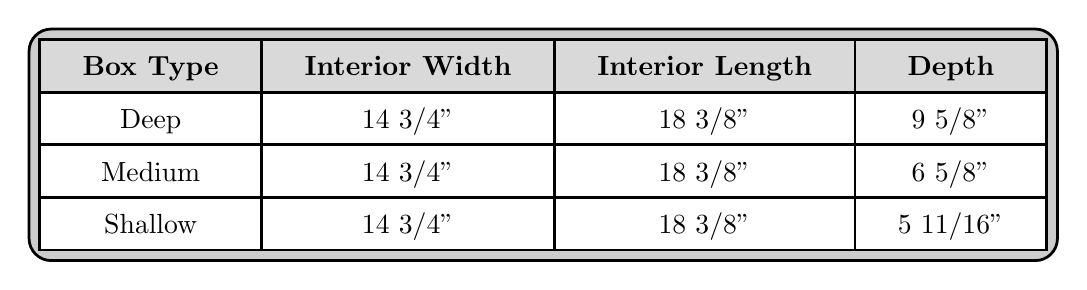
\begin{tikzpicture}
			\node[draw, rounded corners=8 pt, line width=1 pt, fill=black!20] {
				\begin{tabular}{|c|c|c|c|}
					\hline
					\rowcolor{gray!30}
					\textbf{Box Type} & \textbf{Interior Width} & \textbf{Interior Length} & \textbf{Depth} \\
					\hline  
					\rowcolor{white!20}
					Deep & 14 3/4” & 18 3/8” & 9 5/8” \\
					\hline  
					\rowcolor{white!20}
					Medium & 14 3/4” & 18 3/8” & 6 5/8” \\
					\hline  
					\rowcolor{white!20}
					Shallow & 14 3/4” & 18 3/8” & 5 11/16” \\
					\hline
				\end{tabular}
			};
		\end{tikzpicture}
		\label{tab:LANGSTROTH_DIMENSIONS}
	\end{table}
	
	\begin{figure}[H]
		\centering
		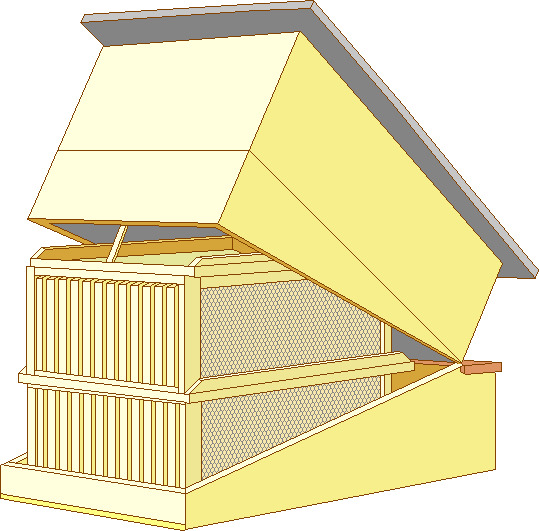
\includegraphics[width=0.4\textwidth]{Images/hive.jpg}
		\caption{Typical Langstroth Hive \cite{CushmanBeeLang}}
		\label{fig:LANGSTROTH_HIVE}
	\end{figure}
	
	\hspace{-0.5 cm}With this in mind, the system shall aspire to:
	\begin{itemize}
		\item Integrate multiple IoT technologies and components into existing beehives, namely sensors, cameras, microphones, motors and scales.
		
		\item Install various AI models for real-time detection and classification, anomaly detection and weather forecasting.
		
		\item Introduce new automated triggers to the hive’s hardware components to allow for swift actions and data-driven decision making.
		
		\item Include a remote monitoring interface for beekeepers to control their hives and monitor different logs, readings or alerts.
	\end{itemize} 
	Markedly, the system shall achieve and meet all its objectives while taking into account the constraints of the fully operational hives around the middle east.
	
	\subsection{Project Overview}
	
	
	The Mele Hive will be concerned with providing domesticated bees with a safe and hospitable habitat while also facilitating the beekeeping process through implementing the following features:
	
	\begin{figure}[H]
		\centering
		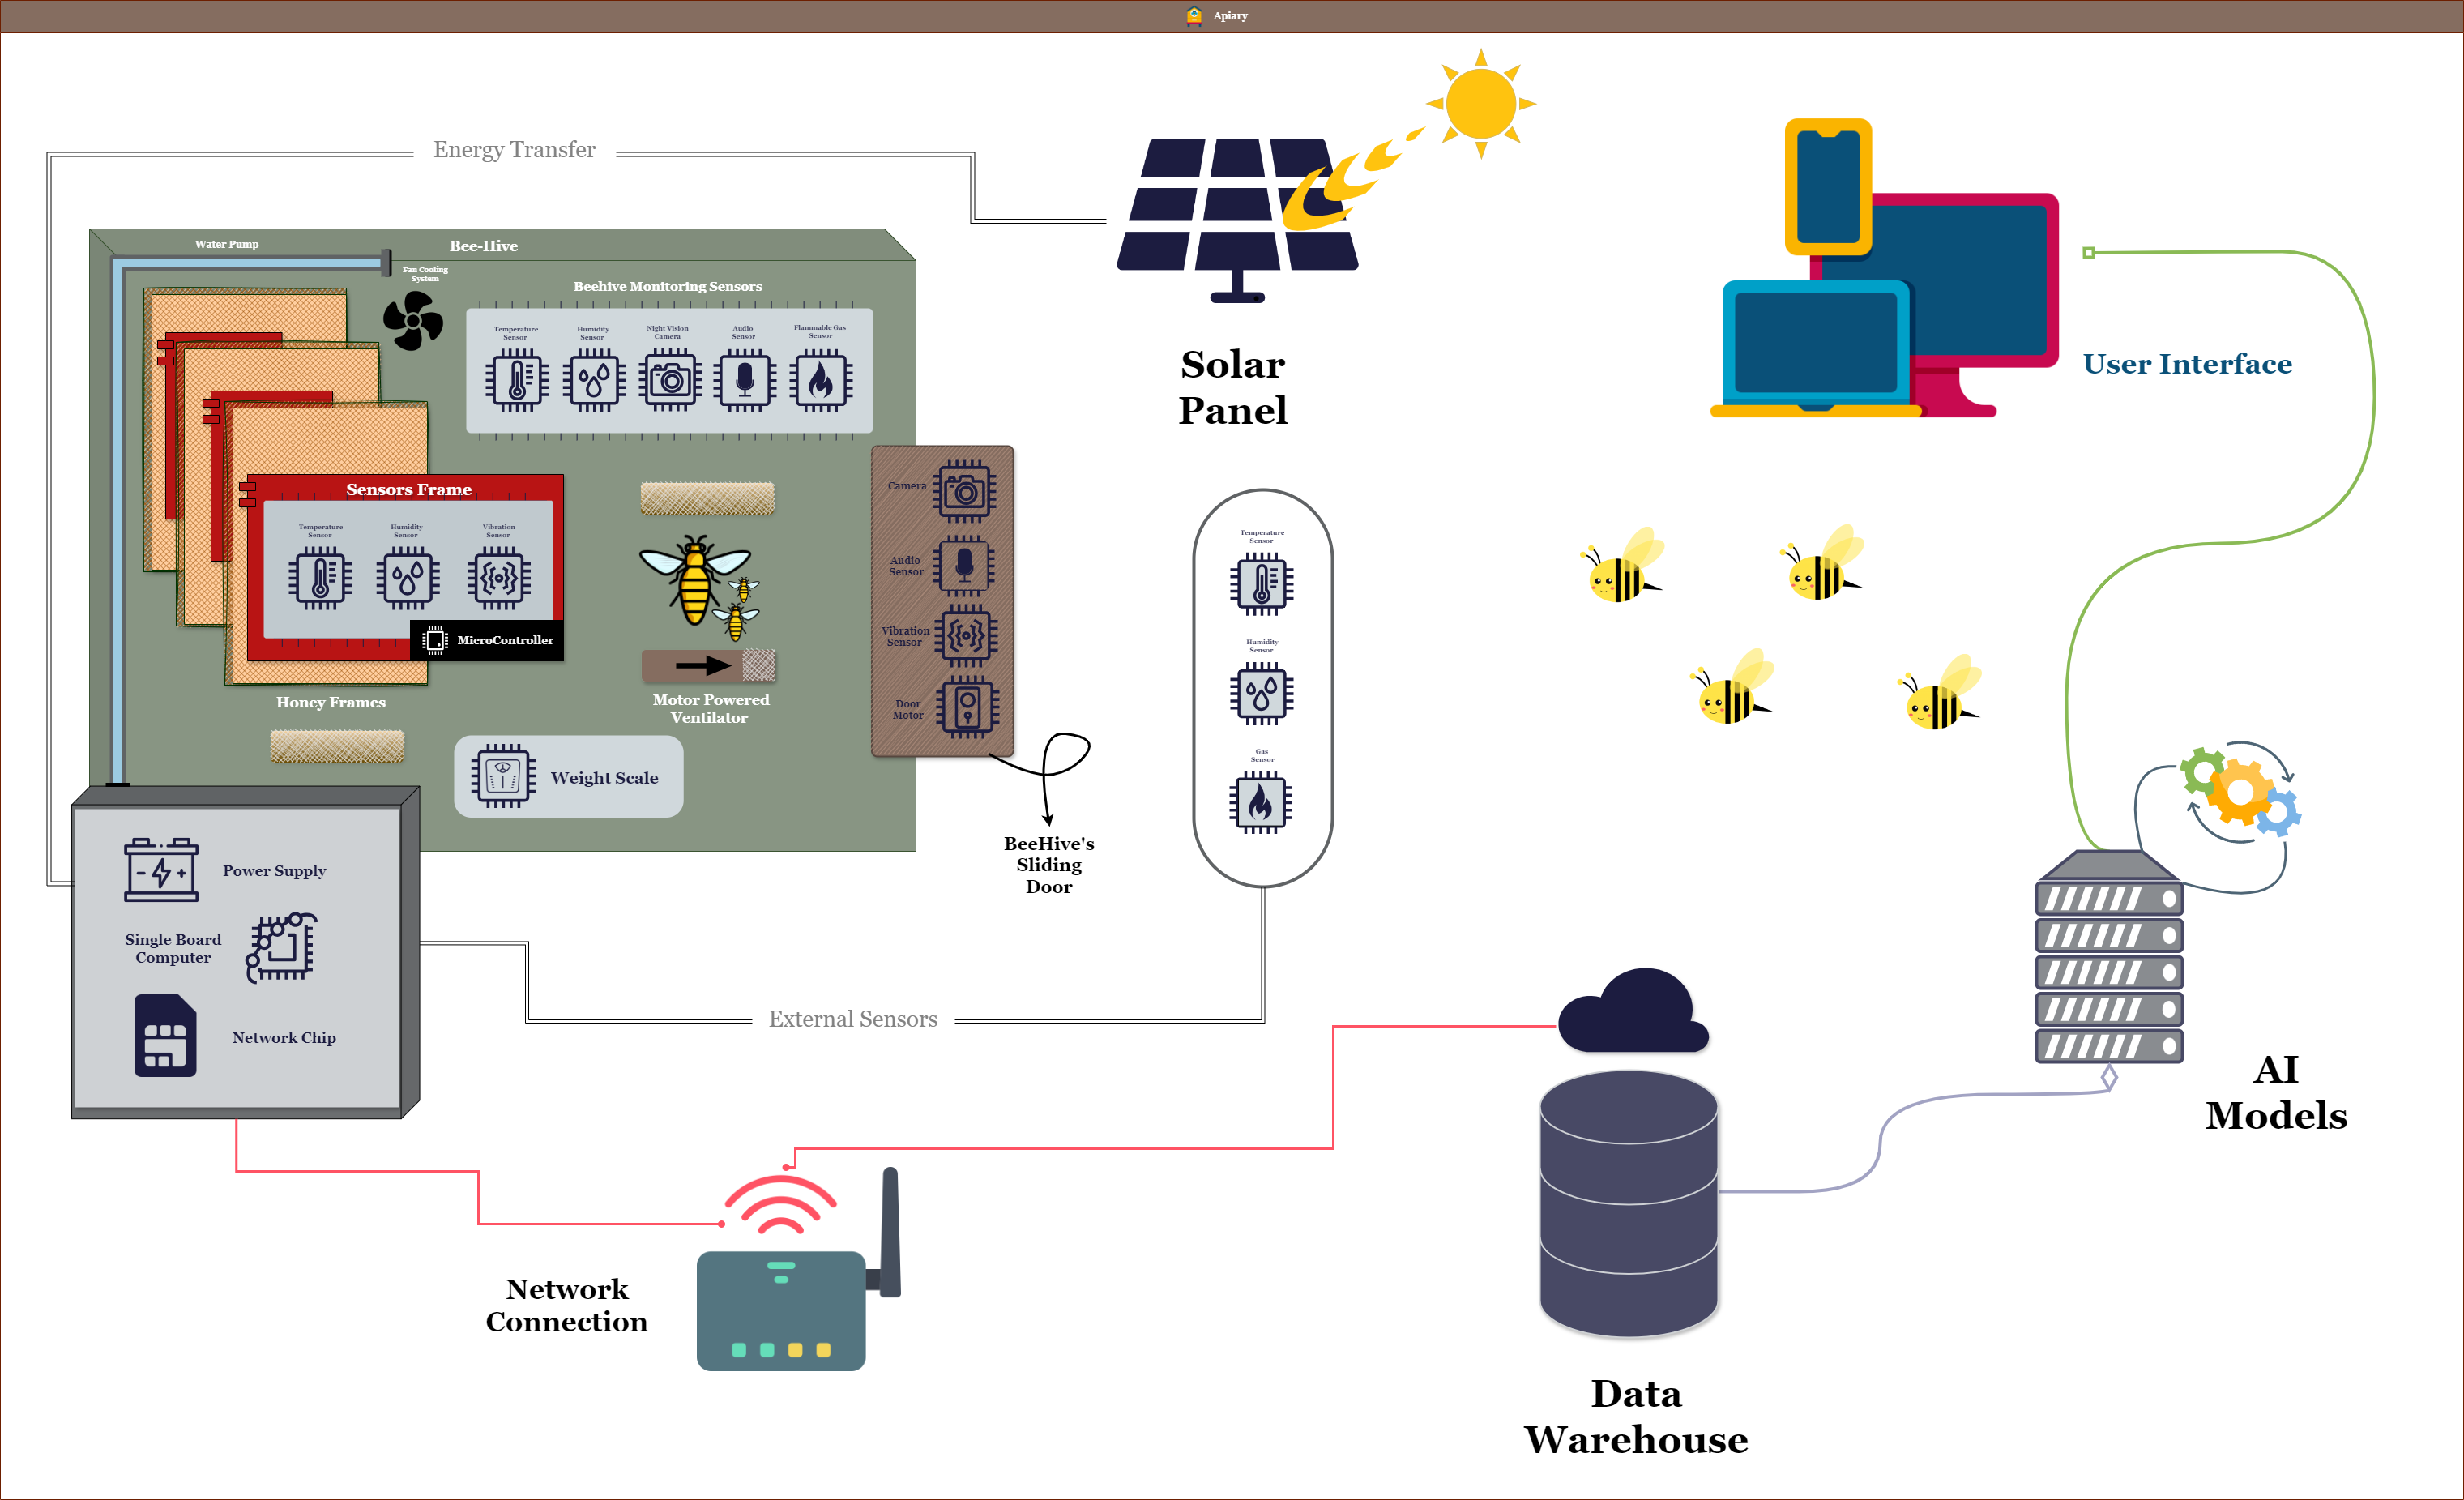
\includegraphics[width=\textwidth]{Images/Diagrams/System Overview.png}
		\caption{Project Overview}
		\label{fig:PROJECT_OVERVIEW}
	\end{figure}
	\vspace{1.5 cm}
	\subsubsection{Temperature and Humidity Monitoring and Control}
	The system sensors will continuously feed their readings into highly competent forecasting models which shall then be used along with weather API data to decide the best course of action to maintain a stable and comfortable environment through activating the internal air cooling system or opening the beehive vents.
	\begin{enumerate}
		\item Capturing temperature and humidity readings.
		\item Forecasting imminent weather conditions.
		\item Integrating forecasts with API data
		\item Selecting best course of action by controlling:
		\newpage
		\begin{itemize}
			\item Vents
			\begin{figure}[H]
				\centering
				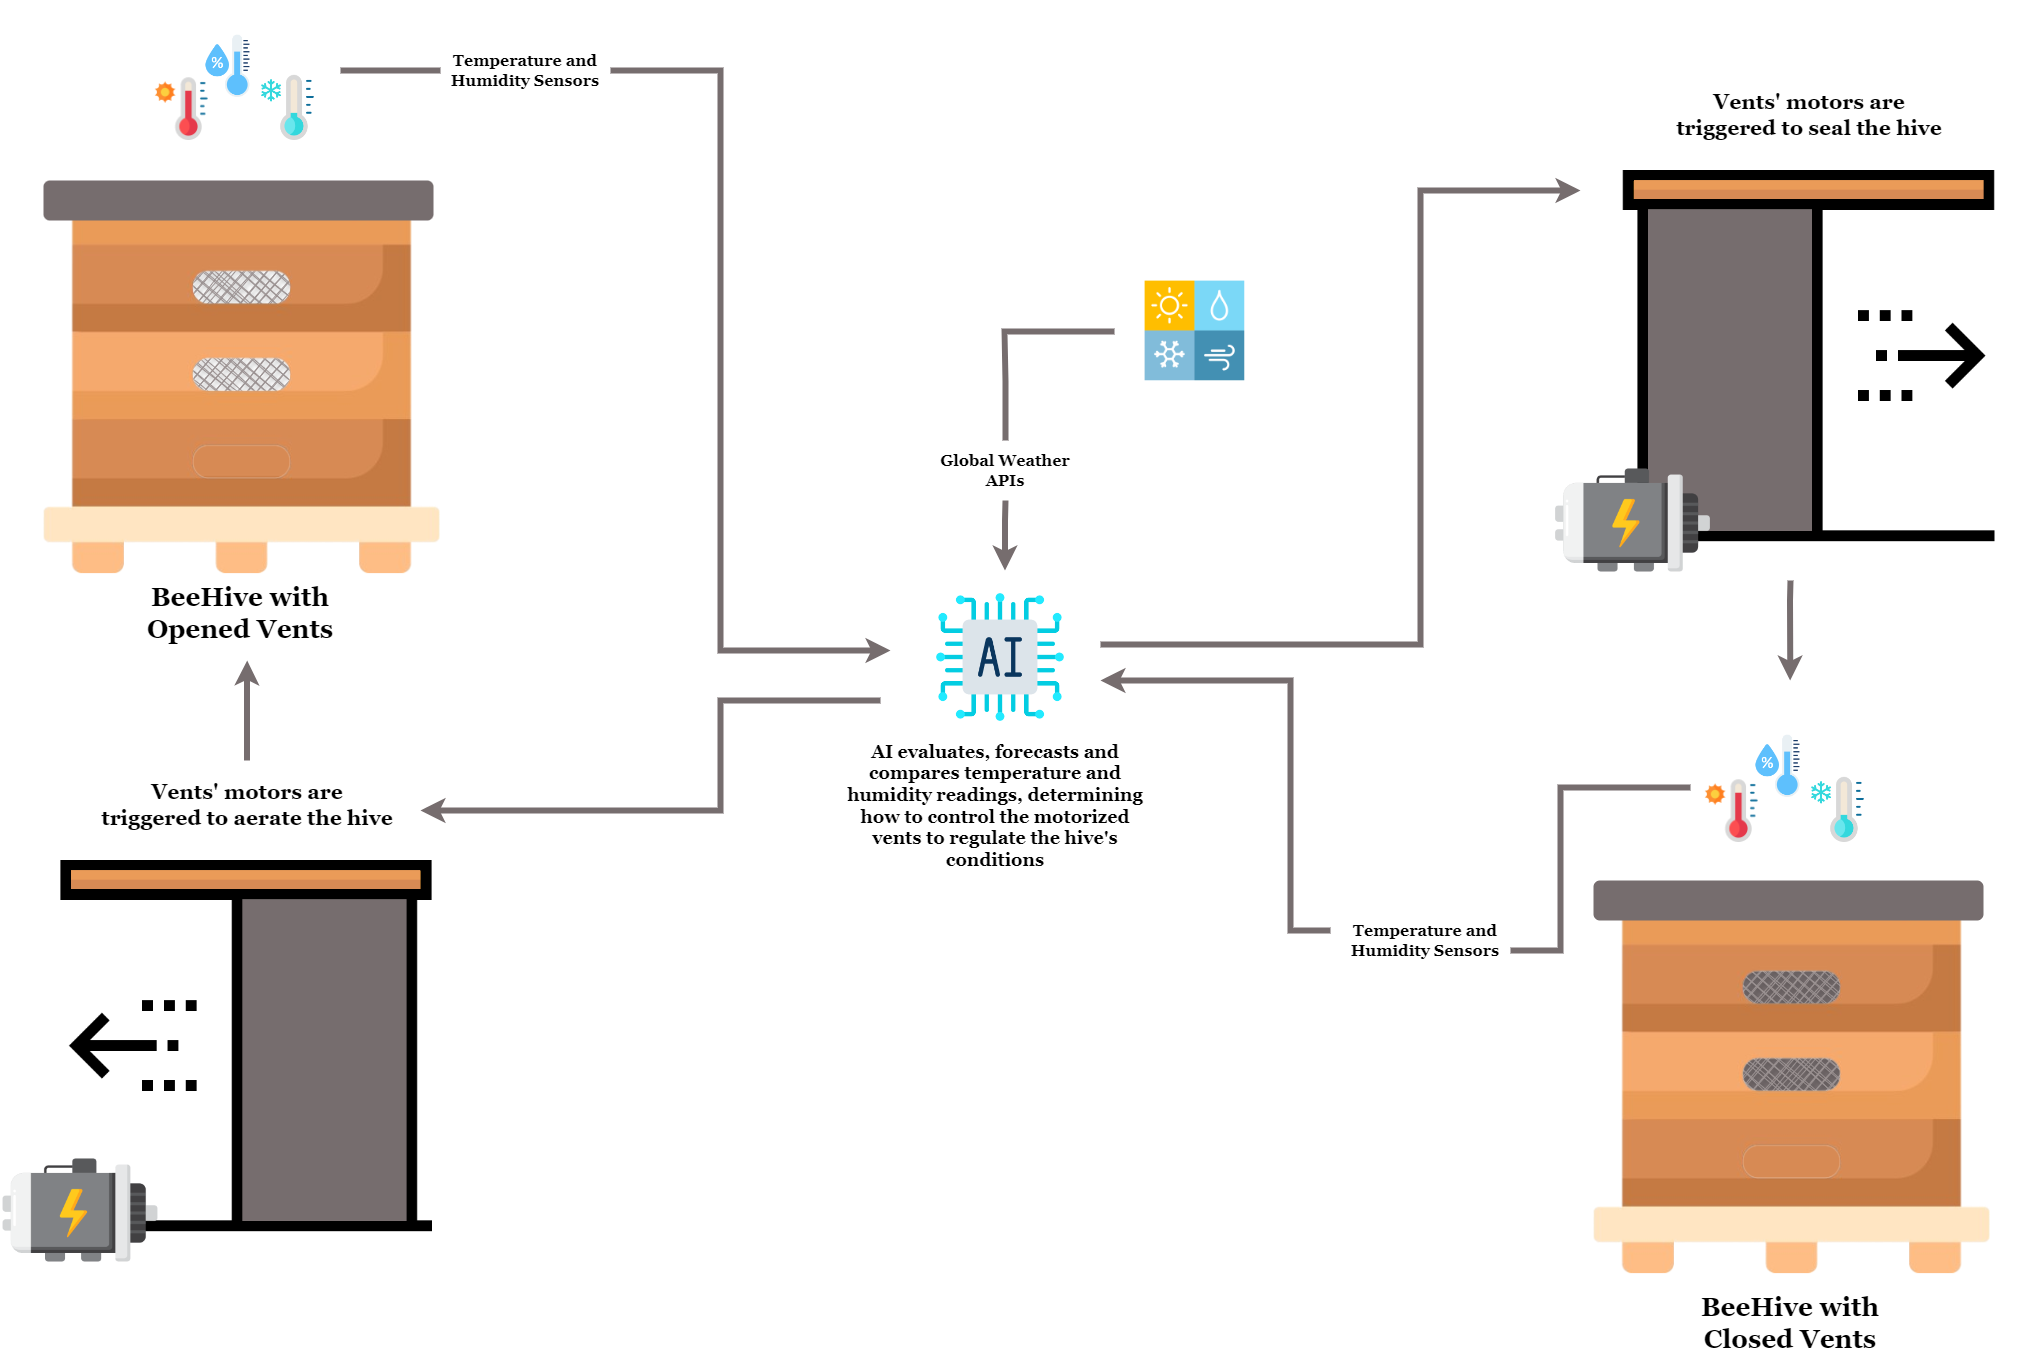
\includegraphics[width=0.5\textwidth]{Images/Diagrams/Vents.png}
				\caption{Vent Automation Sequence Diagram}
				\label{fig:VENTS}
			\end{figure}
			\vspace{1 cm}
			\item Cooling System
			\begin{figure}[H]
				\centering
				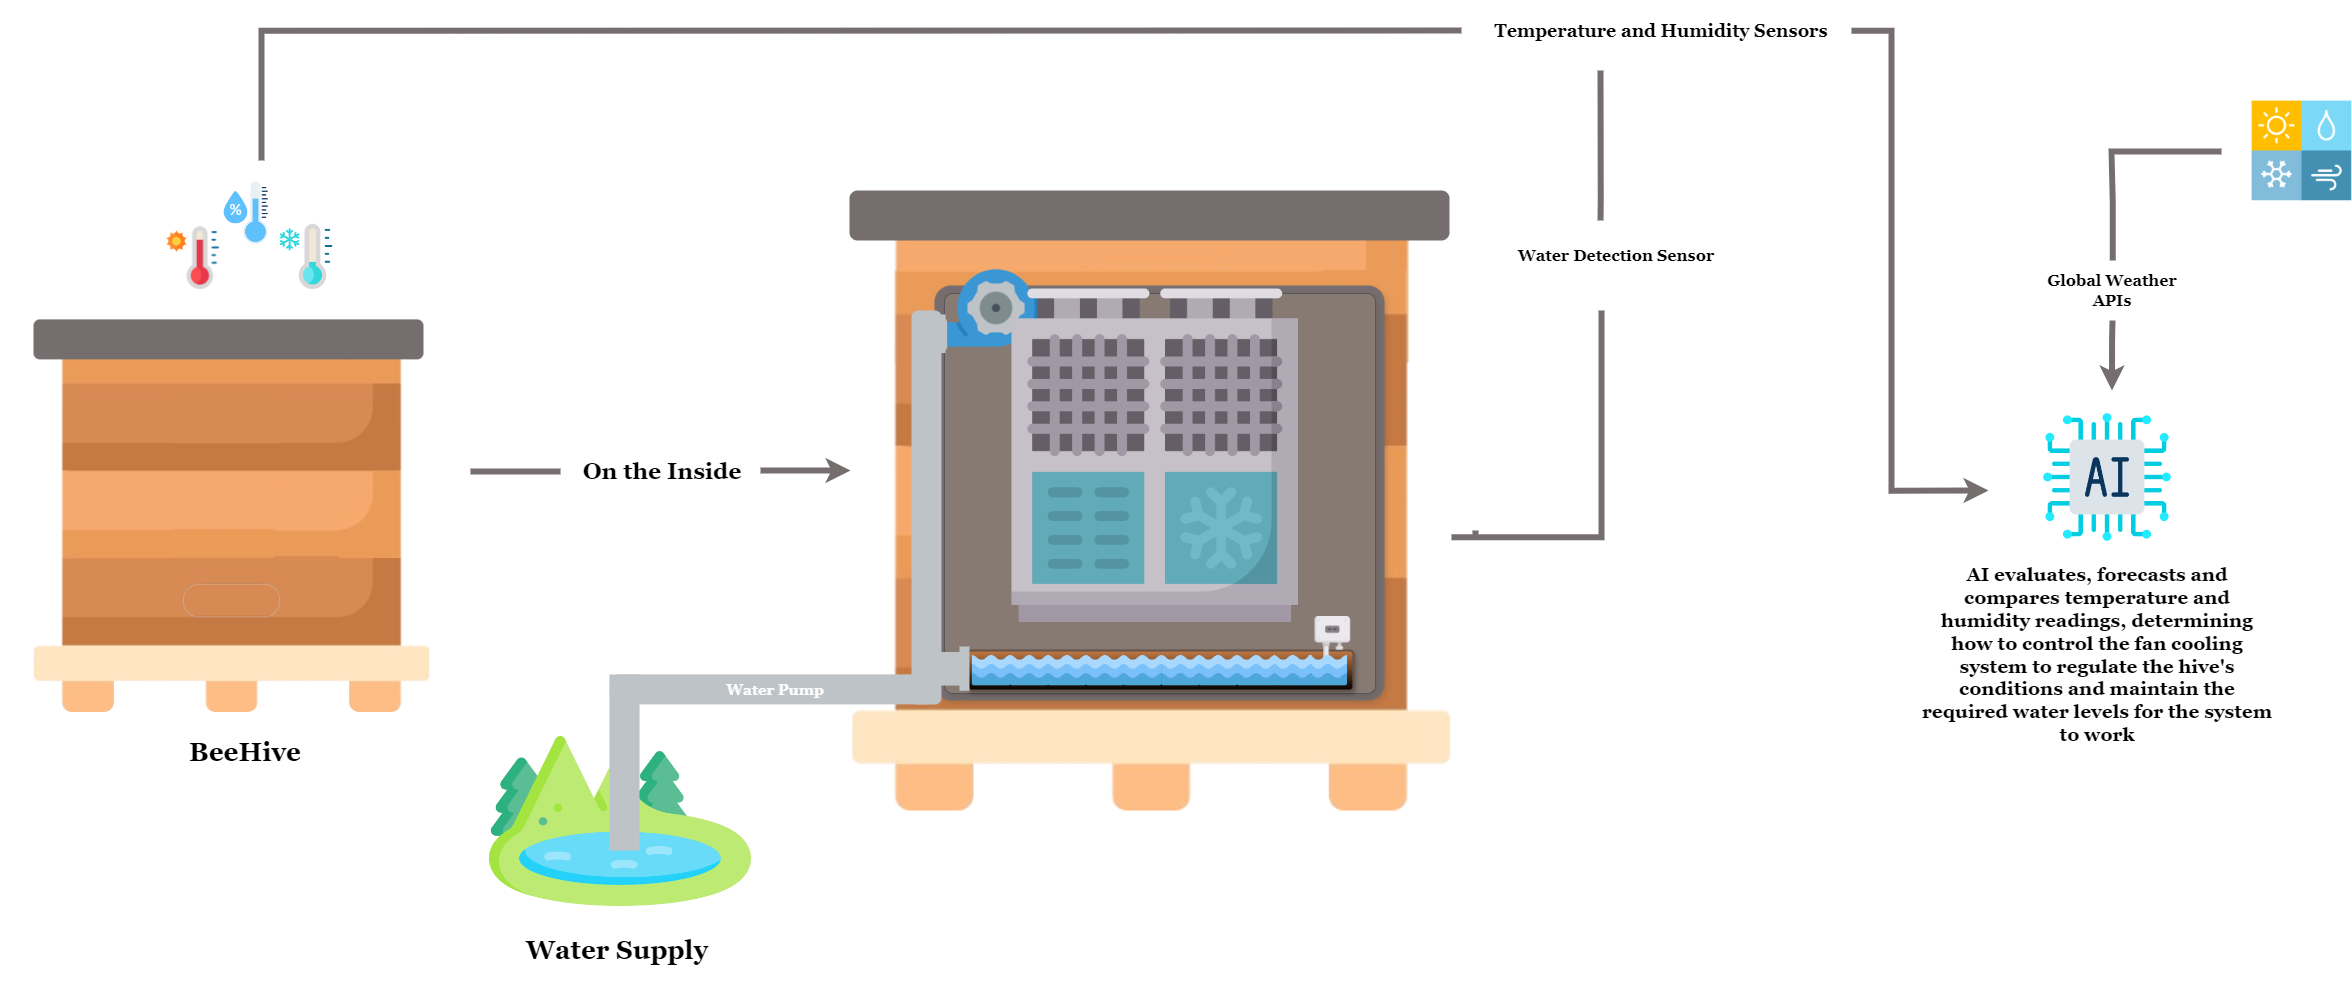
\includegraphics[width=0.5\textwidth]{Images/Diagrams/Cooling System.png}
				\caption{Cooling System Diagram}
				\label{fig:COOLING}
			\end{figure}
		\end{itemize}
	\end{enumerate}
	
	\vspace{1 cm}
	\subsubsection{Honey Yield Tracking}
	Using pinpoint accurate image classification and object detection models accompanied by advanced image processing techniques the internal beehive camera shall be able to distinguish between capped and uncapped honey to notify beekeepers about the percentage of honey ripe for the taking per hive frame. The system shall also be outfitted with an adequate weight sensor to estimate the amount of produced honey.
	\begin{enumerate}
		\item Detecting honeycomb object.
		\item Recognizing whether it is capped or uncapped.
		\item Fetching corresponding weight readings.
	\end{enumerate}
	\newpage
	\subsubsection{Bee Population Monitoring and Behavioral Analysis}
	The Mele system will boast a suite of monitoring tools and diagnostics, including:
	\begin{itemize}
		\item Bee Population Count: 
		Where the system keeps track of bees arriving to and departing from the hive, computing an overall population tally.
		\item Hive Health Monitoring: 
		In which the system keeps watch for possible Varroa mite infestations using internal cameras.
		\item Hive Anomaly Detection: 
		Mainly operates by leveraging vibration sensors to detect any possible irregularities or shift in bee behavior.
	\end{itemize}
	
	\subsubsection{Threat Detection and Mitigation}
	The system shall employ a variety of sensors and contingencies to ensure the safety and security of the beehive inhabitants through implementing a host of safeguards against any possible environmental hazard or malicious entity. The hive security system package will provide: \\
	\begin{itemize}
		\item Flammable Gas Detection:
		The hive comes equipped with flammable gas sensors that alert the beekeepers on picking up traces of high concentrations of volatile gases in the immediate vicinity. \\
		\item Hive Intrusion Prevention System:\\
		Using the on-door camera and mic in addition to highly accurate rapid classification models, the system identifies whether or not the approaching entity is a bee and reacts accordingly deploying special countermeasures specifically when detecting Wasps as they are chiefly the bees' natural predator.
		
		\begin{itemize}
			\item Bee: Open hive door.
			\item Wasp: Close hive door, notify beekeepers and activate defensive measures.
			\item Other insects: Close hive door.
		\end{itemize}
		\begin{figure}[H]
			\centering
			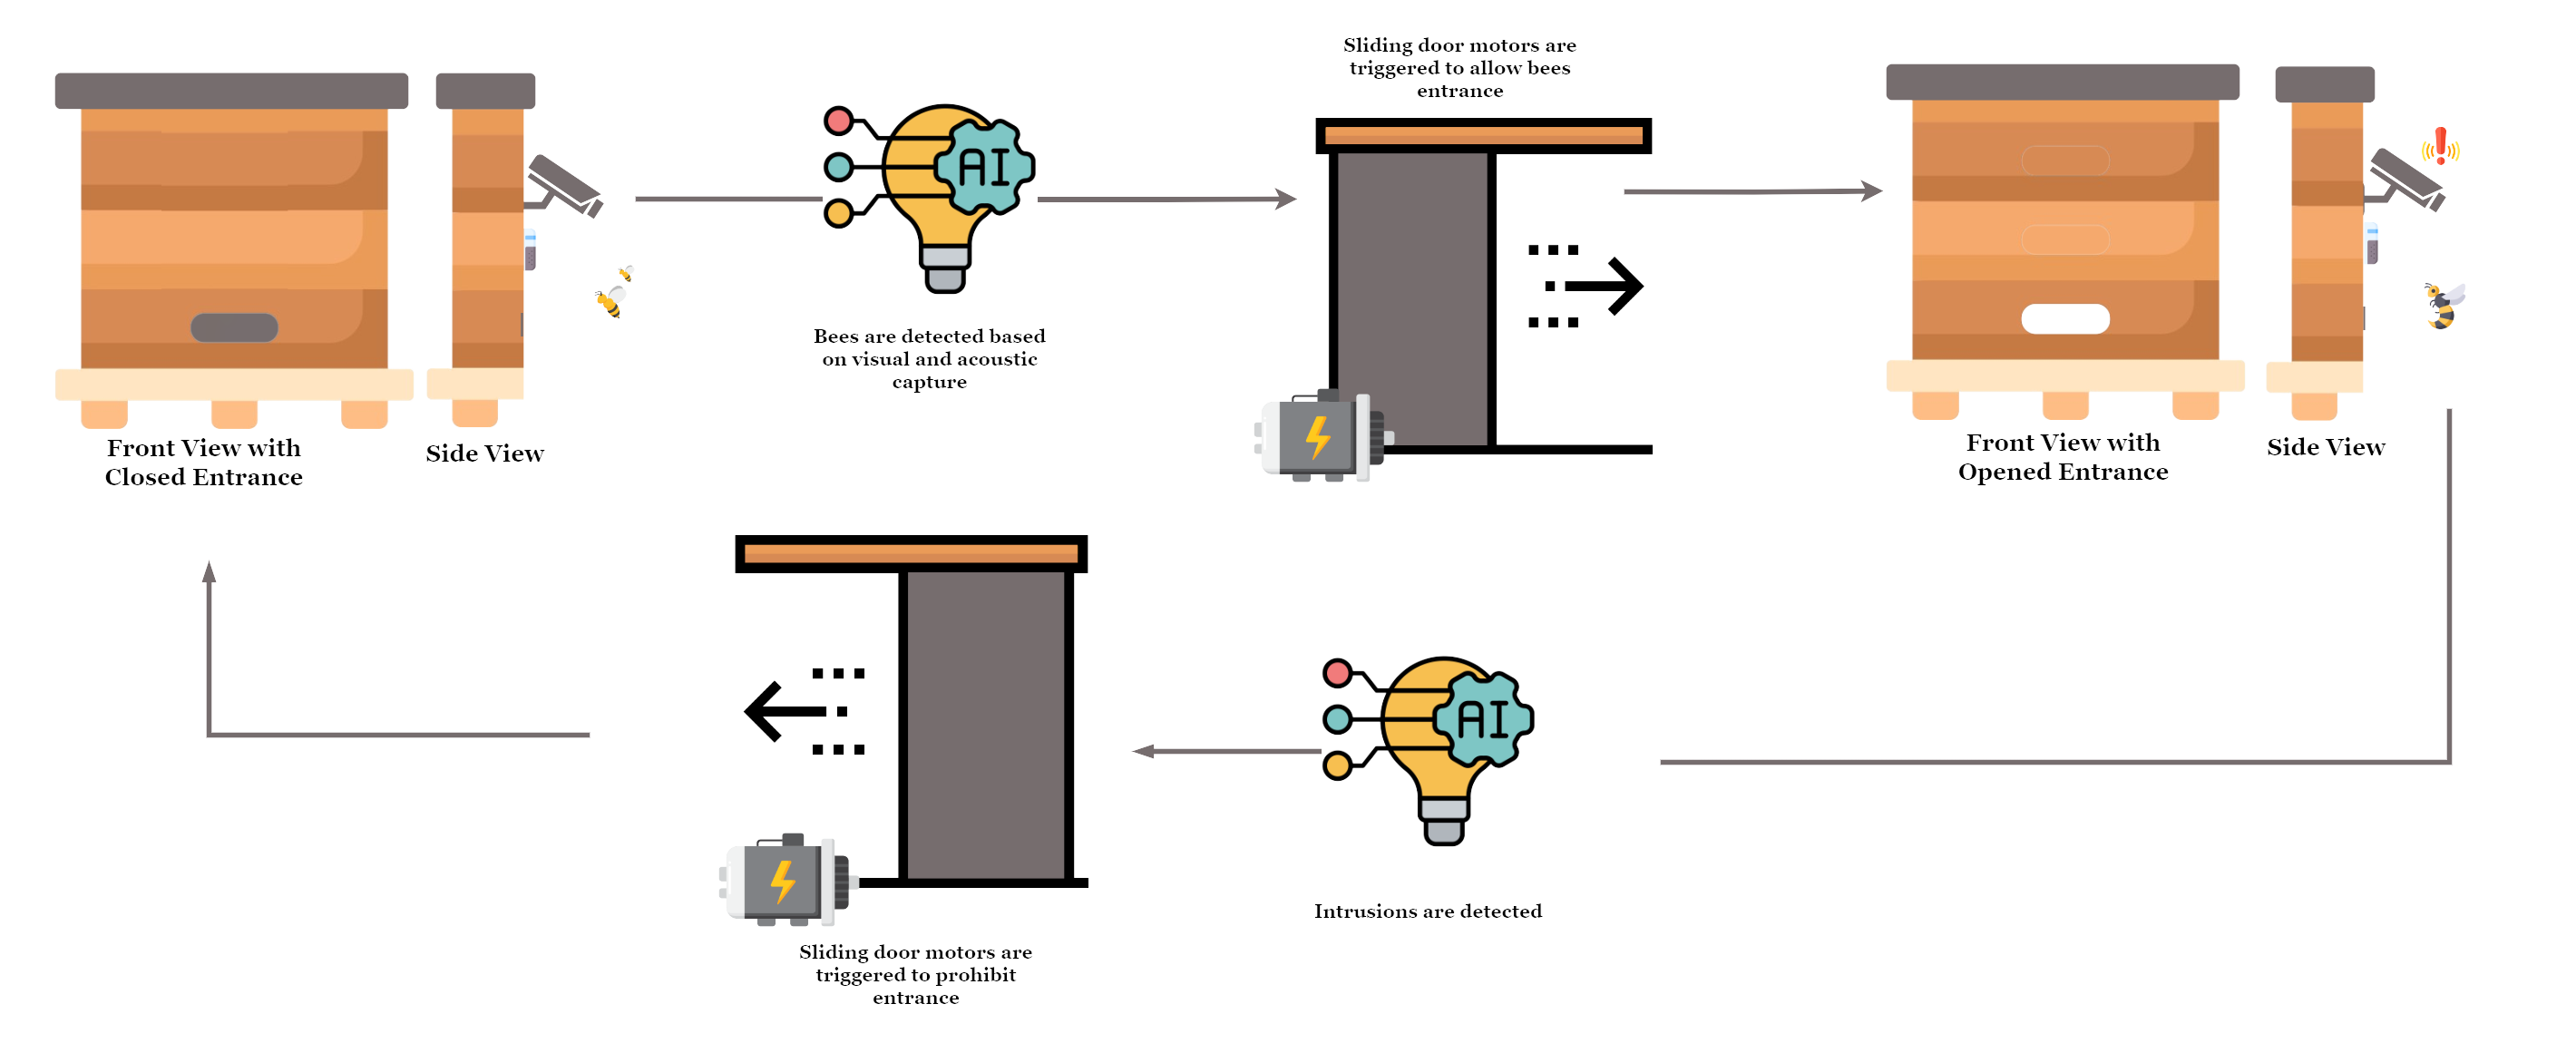
\includegraphics[width=0.7\textwidth]{Images/Diagrams/Motorized Door.png}
			\caption{Door Sequence Diagram}
			\label{fig:DOOR}
		\end{figure}
	\end{itemize}
	
	\subsection{Stakeholder}
	\subsubsection{Internal}
	\begin{itemize}
		\item \textbf{Supervisor}: Dr. Walaa Hassan 
		\item \textbf{Assistant Supervisor}: Eng. Hamsa Mahmoud
		\item Moshir Ashraf \small\textit{(Team Leader)}
		\item Khaled Yehia 
		\item Dalia Raafat
		\item Adam Loay
		\item Mounir Nader
	\end{itemize}
	\subsubsection{External}
	All those interested and affected by bee-keeping practices, more particularly across the middle east. Chiefly, the head of \textbf{"Al-Badran"} bee-keeping group, \textbf{Fouad Mohamed Badran}, who has so graciously lent his time and efforts to support this project.
	
	\section{Similar System}
	\subsection{Academic}
	% 1st paper %
	\noindent \textbf{Stefania Cecchi , Susanna Spinsante , Alessandro Terenzi and Simone Orcioni} \cite{cecchi2020smart} address the widespread decline of honey bee colonies, particularly Colony Collapse Disorder (CCD). The researchers created a multi-sensor  system to monitor weight, sound, temperature, humidity and co2 levels continuously in the hive. Consequently, the system uses all of these data streams to provide insights into the behaviour and health of the bees, thus helping to detect key events like swarming and beehive theft. They collected their own data from hives installed within their university campus over the course of a year. The data included changes in weight, sound, temperature, humidity and co2 levels inside the hive. The researchers showed a demonstration of the system's ability to successfully monitor and detect key events. For instance, they used the changes in weight and sound signatures to accurately detect swarming events. One critical criticism is that the reliability of the dataset is slightly questionable as they noted that humidity sensors provided wrong and missing data for certain months. \\ \newline
	
	
	% 2nd paper %
	\noindent \textbf{Dániel Tamás Várkonyi, Márta Alexy and Tomáš Horváth}\cite{varkonyi2022beyond} discuss unique challenges in a honeybee monitoring project that uses IoT and AI, focusing on issues like trust between beekeepers and researchers, seasonal data collection challenges, and data labeling difficulties. The researchers identified these hurdles and stressed the need for strong communication and understanding with beekeepers. They also looked into hardware limitations and emphasized the importance of contextual information beyond sensor data. Although lacking specific dataset details, the project used hive sensor data to monitor conditions and honey production. The authors categorized these challenges into four main areas, offering insights for future agricultural projects. \\ \newline
	
	
	
	% 3rd paper %
	\noindent \textbf{Andreas KÖNIG} \cite{konig2019indusbee} aimed to address the need for non-invasive hive monitoring systems as traditional monitoring methods are time-consuming and stresses the bee colony. The author created a system that utilized multiple sensors which include temperature sensor, moisture sensor, load cell, camera systems, and microphones. Additionally, the author used machine learning models to classify the hive state using acoustic data collected from the microphones, and also used a two stage procedure involving blob analysis and knn to classify and count the varroa mites. The author collected his own dataset from using all the available sensors. The author's system was successful in classifying hive states with an accuracy of 98\% when using testing data. On the other hand, when the system was tested on a live beehive, it was able to accurately identify hive conditions, but some confusion did occur between different hive states. Moreover, varroa classification and counting worked well in a clean environment with minimal debris and dust. One criticism is that they author didn't mention how the system would perform in a real-world environment where dense debris and dust will be present. \\ \newline 
	
	
	
	% 4th paper %
	\noindent \textbf{Rahman Tashakkori , Abdelbaset S. Hamza and Michael B. Crawford} \cite{tashakkori2021beemon} strove to address the declining bee population due to various factors. This problem is made even worse as traditional hive monitoring methods are inefficient for large-scale apiaries. The authors developed a hive monitoring system that includes audio, video, temperature, humidity and weight sensors  to allow beekeepers to remotely monitor multiple beehives. Additionally the lack of a physical element to the monitoring would reduce the disturbance to the bees while also improving the quality of the data. Furthermore, they used CNNs to distinguish bee sounds from other sounds in the background. They determined that CNNs were better than traditional machine learning models for this particular case as a result of their previous research .Moreover, the researchers collected their own dataset by continuously recording video audio and environmental data. The system proved capable of collecting real-world data in addition to being able to track bee traffic, and hive status without causing any disruptions to the bees. However, something which can't be overlooked is the fact that they mention audio and video analysis, but they don't mention detailed methods or results of these components. \\ \newline
	
	
	
	% 5th paper %
	\noindent \textbf{Elias Ntawuzumunsi, Santhi Kumaran and Louis Sibomana} \cite{ntawuzumunsi2021self} tackle low honey production and colony loss resulting from unmonitored hive conditions, such as temperature and humidity. The authors proposed a self-powered monitoring system that continuously monitors temperature, humidity, and weight inside the hive and regulates them automatically. Temperature and humidity inside the hive are regulated using an electric fan and a thermoelectric heater. Furthermore, the system harvests energy using piezoelectric transducers to collect energy from vibrations, and the system uses RF energy harvesting devices to convert electromagnetic energy into direct current. The researchers collected data through real-time monitoring of conditions inside the hive. Their results showed that the system was able to successfully regulate the hive temperature between 32-36 degrees Celsius. In addition, the system was able to harvest enough power to run the monitoring system without external power. One criticism is that their energy harvesting method might prove inadequate in conditions where bee activity is reduced, thus further field testing is necessary.\\ \newline
	
	
	
	% 6th paper %
	\noindent \textbf{Julian Marstaller, Fredrick Tausch,and Simon Stock}
	\cite{marstaller2019deepbees} introduce \textbf{DeepBees}, a system using computer vision and deep learning to monitor honeybee health amid population declines. With a dataset covering genus classification, pollen detection, and pose estimation, the system outperformed single-task models, boosting classification AUC from 70.34\% to 82.41\%. Improvements could include tackling data imbalance, testing across species and environments, and adding temporal analysis for deeper insights. Visuals clearly illustrate the architecture and results. \newpage
	
	% 7th paper %
	\noindent \textbf{H A Rosli, N Abdul Malik and Y A Ahmad} \cite{rosli2022iot} tackle the challenge of efficiently monitoring stingless bee colonies, traditionally managed through time-consuming manual inspections. The authors introduced an IoT-based solution that employs various sensors—measuring temperature, humidity, weight, and pressure—to collect data in real time. This setup enables beekeepers to track hive conditions remotely. Sensor readings, recorded every 15 seconds, are uploaded to a cloud platform for analysis. The results confirmed effective monitoring of critical parameters like temperature, humidity, and weight, offering valuable insights into the colonies' health. However, the paper could be improved by discussing the limitations of relying solely on continuous Wi-Fi for data transmission. A GSM module could be a more reliable alternative. Figures detailing the system's architecture and findings are presumably included in the full study.\\ \newline
	
	
	% 8th paper %
	\noindent \textbf{Dimitrios I. Kiromitis , Christos V. Bellos, Konstantinos A. Stefanou, Georgios S. Stergios Thomas Katsantas  and Sotirios Kontogiannis} \cite{kiromitis2022bee} address in this paper the need for a reliable beehive monitoring system that can provide real-time insights into bee behavior and environmental conditions, as traditional methods are manual and often inadequate. The researchers developed the Bee Sound Detection (BeeSD) system, which combines temperature, humidity, and sound sensors within an IoT device for continuous monitoring and cloud-based data transmission. The study successfully demonstrates the system’s capabilities, establishing key performance indicators such as low energy consumption, ease of installation, and affordability. However, it falls short in providing detailed dataset transparency and user feedback, which could strengthen the findings. The paper includes figures that detail the system architecture and components, highlighting the innovative features of the BeeSD design. \\ \newline 
	
	
	% 9th paper %
	\noindent \textbf{Nebojša Andrijevi, Vlada Uroševi, Branko Arsi, Dejana Herceg and Branko Savi } \cite{andrijevic2022iot} address the declining honeybee population and the instability in their ecosystem due to changes in the environment, diseases, and human activity. The authors developed a system to monitor the hive's condition using sensors that include temperature,humidity and air quality. Additionally, they used ARIMA, Facebook prophet, and Long Short-term memory (LSTM) to help in forecasting bee activity patterns which can indicate threats of abnormal conditions. Moving on, the researchers collected their own dataset over 20 days in October of 2021. The dataset focused on hive conditions externally and internally at 5 minute intervals which are later on combined into hourly averages. Furthermore, the dataset had the usual data points like temperature, humidity, air quality, but curiously they also collected light intensity and UV levels to analyze bee behavior under different environmental factors. The researchers concluded that the LSTM model outperformed the others, and in addition, the system effectively was able to capture trends in bee activity predict bee movement patterns based on environmental factors accurately. One criticism is that the testing was only conducted during the fall so it might not be fully capable of representing bee behavior year-round. \\ \newline 
	
	
	% 10th paper %
	\noindent \textbf{Andrzej Szczurek , Monika Maciejewska ,and Piotr Batog} \cite{szczurek2023monitoring}
	explore challenges in urban beekeeping, focusing on real-time hive monitoring systems to track conditions and environmental factors. Researchers developed a system with multi-sensor devices, weight scales, and cameras to observe hive atmosphere variations in real-time. Data on temperature, humidity, CO2, VOCs, and particulate matter showed distinct differences between the hive environment and surrounding air, with daily weight and condition changes clearly captured, helping beekeepers manage their colonies. While effective, the paper could benefit from discussing tech limitations, comparing existing systems, and addressing sustainability and cost. Visuals highlight air composition and weight variations relative to environmental factors. \\
	
	% summary table %
	\subsubsection{Summary:}
	\vspace{0.5 cm}
	\begin{table}[H]
		\centering
		\caption{Similar Academic Work Summary}
		\vspace{0.25 cm}
		\resizebox{0.8\textwidth}{!}{%
			\begin{tabular}{|>{\centering\arraybackslash}m{2 cm}|m{6 cm}|m{6 cm}|}
				\hline
				\textbf{Reference} & \textbf{Proposed} & \textbf{Findings} \\ \hline
				% 1st Paper %
				{\cite{cecchi2020smart}} & A system that uses various sensors to provide insights into bee behaviours to help detect events like swarming and hive theft. & The system successfully detected key events like swarming by using weight info and analyzing bee sounds. \\ \hline
				
				% 2nd Paper %
				{\cite{varkonyi2022beyond}} & IoT and AI-based honeybee monitoring system designed to gather hive data and address challenges like trust with beekeepers, seasonal data variability, and labeling difficulties. & Strong communication with beekeepers and additional contextual information beyond sensor data are essential for accurate monitoring. \\ \hline
				
				% 3rd Paper %
				{\cite{konig2019indusbee}} & A system that uses sensors, camera systems, microphones, and ML models to classify hive state. & The system proved accurate in its classification both when using testing data and in a real-world scenario. \\ \hline
				
				% 4th Paper %
				{\cite{tashakkori2021beemon}} & A system that monitors hive conditions remotely using sensors and uses CNNs for audio classification. & The system proved capable of collecting data and tracking the hive status without disrupting the bees. \\ \hline
				
				% 5th Paper %
				{\cite{ntawuzumunsi2021self}} & A self-powered system to monitor and regulate hive conditions using various sensors, a fan, and a thermoelectric heater. & The system was able to gather enough power to run the monitoring system without any external power, and it was able to keep the temperature between 32-36°C. \\ \hline
				
				% 6th Paper %
				{\cite{marstaller2019deepbees}} & DeepBees, a computer vision and deep learning system designed to monitor honeybee health in response to declining populations. & DeepBees significantly outperformed single-task models, increasing classification AUC from 70.34\% to 82.41\%. \\ \hline
				
				% 7th Paper %
				{\cite{rosli2022iot}} & IoT-based monitoring system for stingless bee colonies to replace time-consuming manual inspections. & The system effectively monitors crucial hive conditions, providing beekeepers with valuable health insights. \\ \hline
				
				% 8th Paper %
				{\cite{kiromitis2022bee}} & BeeSD, IoT-based solution for real-time beehive monitoring that tracks bee behavior and environmental conditions using temperature, humidity, and sound sensors. & BeeSD performs well in energy efficiency, ease of setup, and affordability. \\ \hline
				
				% 9th Paper %
				{\cite{andrijevic2022iot}} & A system that makes use of sensors and different forecasting models to forecast bee activity patterns. & The system captured trends in bee activity and successfully predicted the movement patterns of bees. \\ \hline
				
				% 10th Paper %
				{\cite{szczurek2023monitoring}} & A real-time monitoring system for urban beekeeping, using multi-sensor devices, weight scales, and cameras to track hive conditions and environmental factors. & Findings suggest the system is effective for real-time monitoring, though improvements could include addressing technology limitations. \\ \hline
				
			\end{tabular}%
		}
		\label{tab:SUMMARY}
	\end{table}
	\subsection{Business Applications}
	
	\subsubsection{SAMS}
	The International Partnership on Innovation in \textbf{S}mart \textbf{A}piculture \textbf{M}anagement \textbf{S}ervices is a multi-national project, created with the intention of improving beekeeping practices in tropical regions by combining multiple \textit{IoT} technologies with\textit{ ICT} systems \cite{sams_project_overview}. The project is entirely open-sourced and accessible with multiple technical implementations available on their \href{https://github.com/sams-project}{\textbf{\textit{github}}: \textit{\small sams-project}}. \textbf{SAMS} innovations received appraisal and funding from the \textit{European Union´s Horizon 2020 research and innovation programme}{\footnotesize, under Grant Agreement N 780755,} for their collaboration with multiple partners across Austria, Ethiopia, Germany, Indonesia and Latvia.\\ \newline
	\begin{figure}[H]
		\centering
		
\includegraphics[width=0.38\textwidth]{Images/Simillar/sams-logo.png}
		\caption{SAMS Logo \cite{sams_project}}
		\label{fig:SAMS_LOGO}
	\end{figure}
	\hspace{-0.62cm}The project succeeded in achieving manifold outcomes that enhance beekeeping practices through the integration of multiple technologies. Perhaps, the most significant out of these advances are \cite{sams_project_results} :
	\begin{itemize}
		
		\item \textbf{SAMS Monitoring System}: The team at SAMS partnered and worked aside multiple universities and experts to develop and apply a fully functional monitoring system. The team developed a frame sensor case that integrates temperature, weight, humidity, and audio frequency sensors that can easily be placed within the brood combs, coupled with a weight scale positioned beneath the hive.
		
		\begin{figure}[H]
			\centering
			\begin{minipage}{0.5\textwidth}
				\centering
				\reflectbox{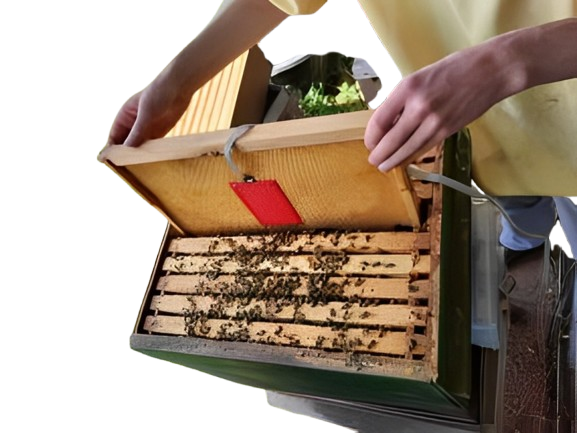
\includegraphics[width=0.8\textwidth]{Images/Simillar/hooked sensor frame.png}}
				\caption{SAMS Sesnor Frame \cite{sams_project_results}}
				\label{fig:SAMS_HOOKED_FRAME}
			\end{minipage}  
			\hfill
			\begin{minipage}{0.45\textwidth}
				\centering
				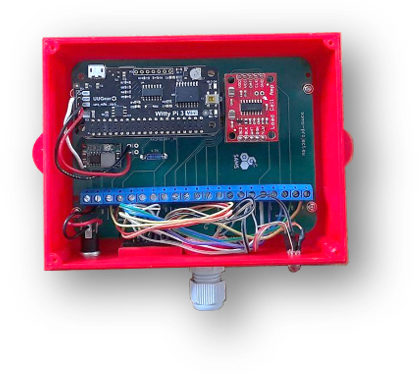
\includegraphics[width=0.4\textwidth]{Images/Simillar/sams sensor case.png}
				\vfill
				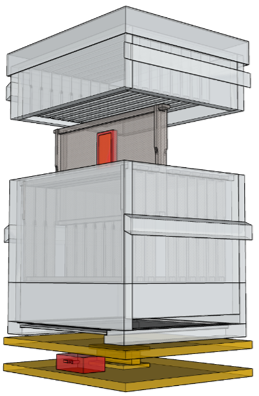
\includegraphics[width=0.4\textwidth]{Images/Simillar/sams hive.png}
				\caption{SAMS Hive and Sensor Case \cite{sams_project_material}}
				\label{fig:SAMS_HIVE}
			\end{minipage}
		\end{figure}
		\item \textbf{SAMS Knowledge Hub – \href{https://wiki.sams-project.eu/index.php/Main_Page}{\small SAMSwiki}}: An \textit{open-sourced} knowledge sharing platform dealing with bees and beekeeping globally. The platform mainly features databases from \textit{Ethiopia} and \textit{Indonesia} all of which are available in \textit{Amharic}, \textit{Bahasa} and \textit{English}. So essential for supporting continuity and accessibility of research, not only does \textbf{SAMSwiki} offer researchers with a comprehensive repository of beekeeping knowledge but it also includes all their project data and results, facilitating broader understanding and engagement in apiculture research. \vspace{0.5 cm}
		
		\item \textbf{SAMS Decision Support System – DSS}:
		A collection of critical tools designed to assist beekeepers in integral decision-making. The \textit{DSS} collects data from various integrated sensors across the hive to detect bees health and colony condition. The system then offers alerts and actionable insights to support real-time data analysis and responsive notifications and triggers. The system also allows for remote control and monitoring via a web-based user interface.
		\begin{figure}[H]
			\centering
			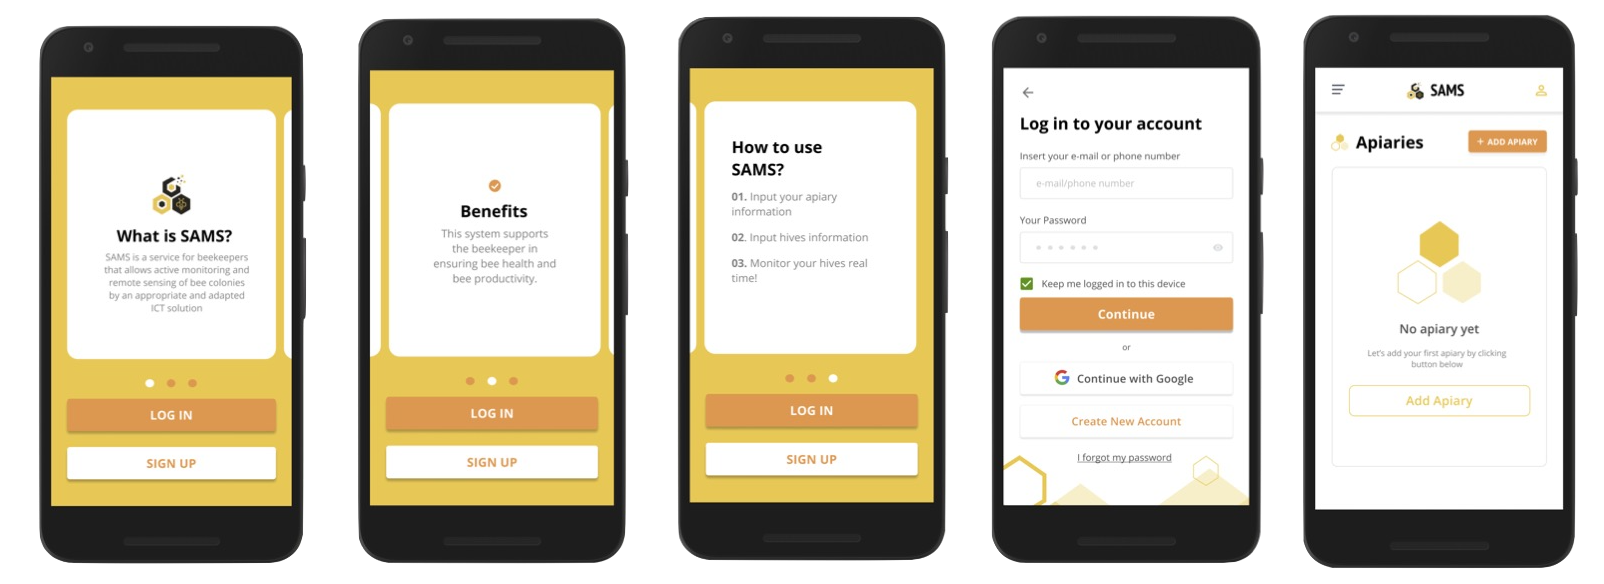
\includegraphics[width=0.5\textwidth]{Images/Simillar/Interface_DSS_old.png}
			\caption{SAMS DSS Interface \cite{sams_figma_design}}
			\label{fig:SAMS_DSS}
			\vspace{0.5 cm}
		\end{figure}
		\item \textbf{SAMS Data Warehouse – DW}: A cloud-based platform that facilitates data storage, access and monitoring. With the addition of various transfer \textit{API}s, the \textbf{DW} served as a communication conduit between the hive's components and their collected data and the beekeeper's \textbf{DSS} interface. The information gathered is uploaded and saved on the \textbf{DW} which their knowledge hub utlizies and provides user access to enable further re-accessing and analytical insights.
		\begin{figure}[H]
			\centering
			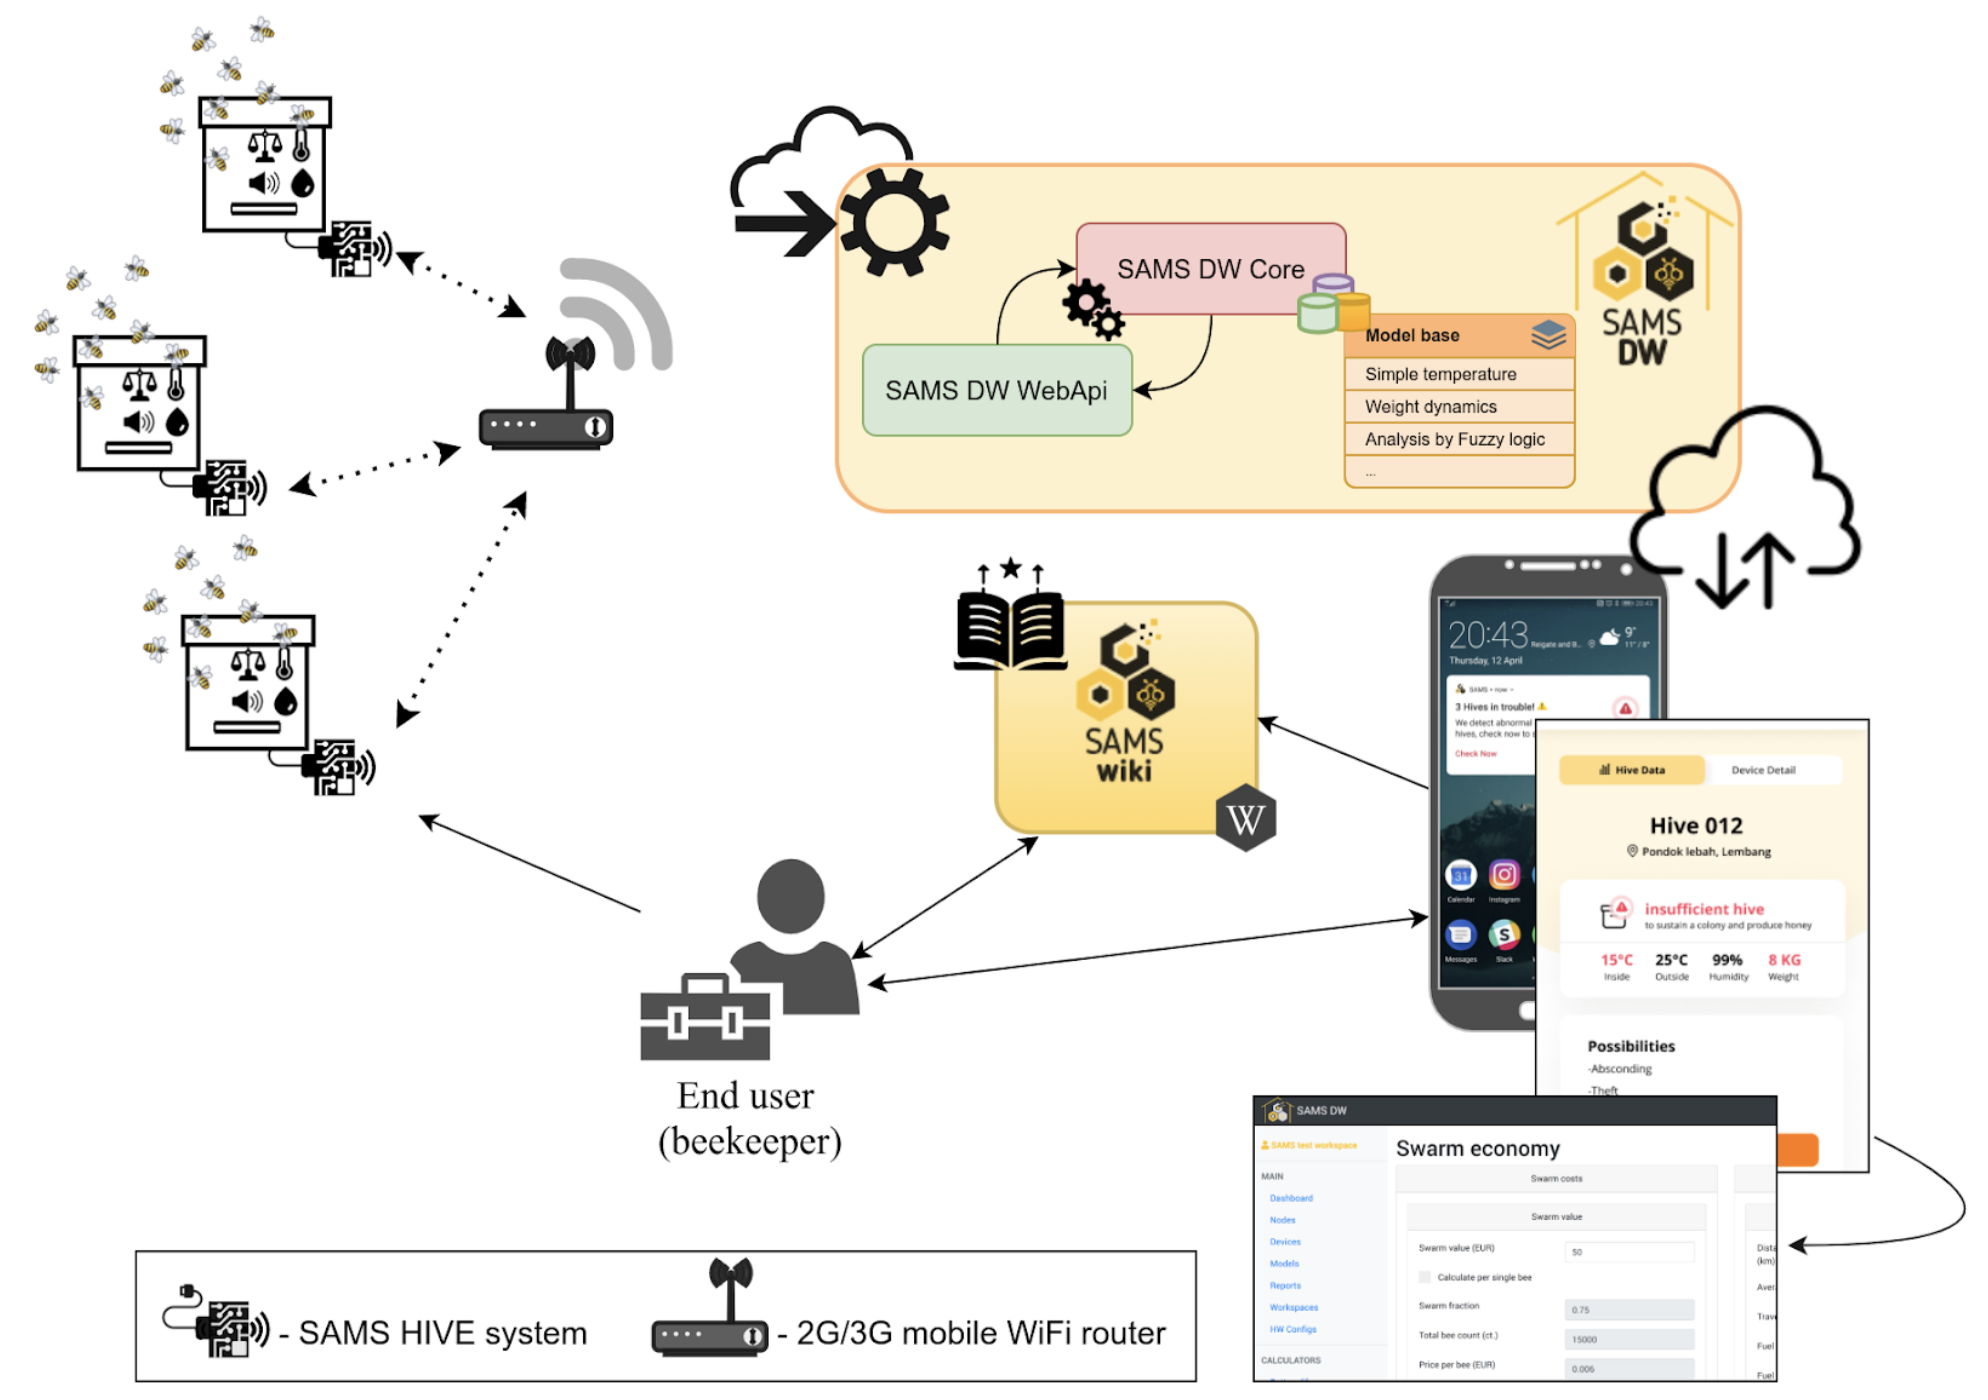
\includegraphics[width=0.6\textwidth]{Images/Simillar/interface_comm.png}
			\caption{SAMS DW Communication \cite{sams_project_results}}
			\label{fig:SAMS_DW}
		\end{figure}
	\end{itemize}
	
	\subsubsection{BeeSage}
	A Netherlands based company which provides standalone , easy to install Smart Beehive Scales that actively monitor beehive location, weight and surrounding temperature conditions \cite{Beesage}. The system presents all relevant data and alerts to users via a user-friendly visually appealing web app to aid beekeepers in maximizing production during peak blooming periods. The company aims to further expand their arsenal of monitoring solutions with their up and coming HiveNode project which will track in-hive temperature and humidity along with live sound monitoring.
	\begin{figure}[H]
		\centering
		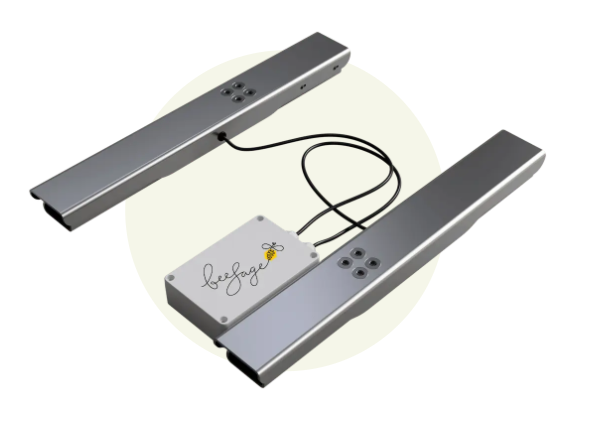
\includegraphics[width=0.4\textwidth]{Images/Simillar/BeeSage_scales.png}
		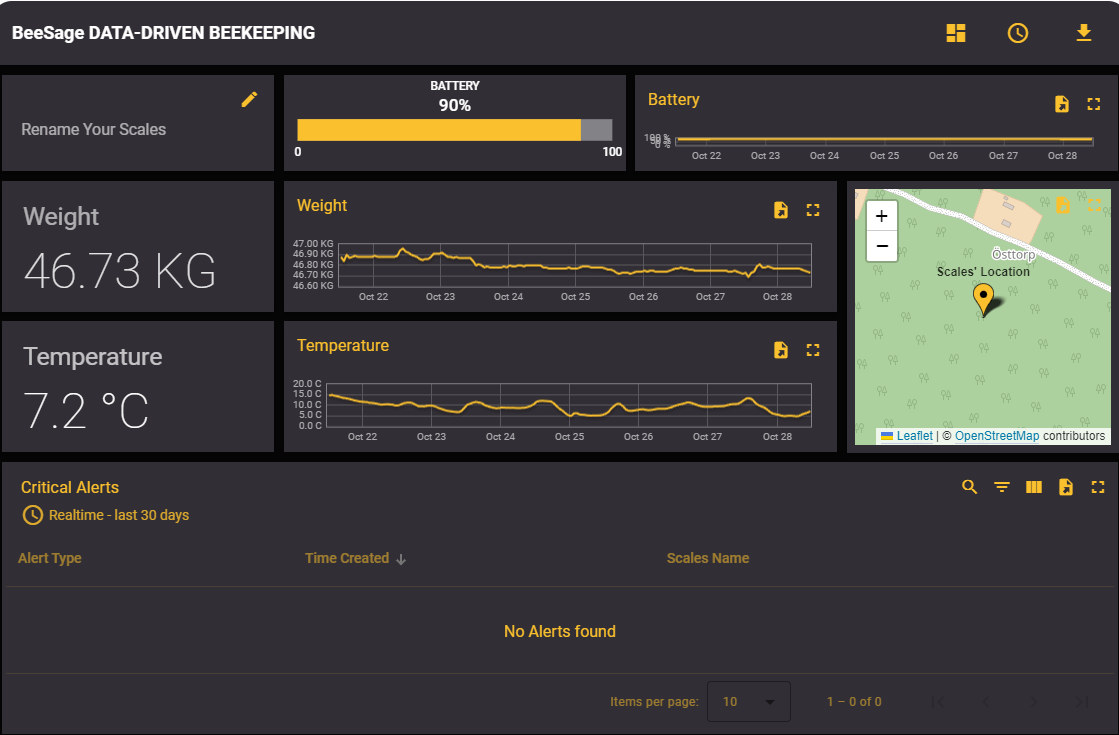
\includegraphics[width=0.4\textwidth]{Images/Simillar/BeeSage App.png}
		\caption{BeeSage Smart Scales and Web App \cite{Beesage}}
		\label{fig:BEESAGE_SCALES}
	\end{figure}
	
	\subsubsection{Apiago}
	A French start-up spearheaded by 3 founders passionate about biodiversity and new technologies, Apiago aims to give all it's customers a shot at beekeeping regardless of their level of knowledge by supplying them with their custom-made fully automated beehives\cite{Apiago}. The Apiago beehive is specifically engineered to be mounted overhead giving it the ability to be deployed in unconventional and tight spaces. The smart beehive is equipped with numerous sensors including but not limited to weight, temperature and hygrometry sensors which are then used to brief the hive owner about current hive health and status in addition to access to the Beekeeper network if further help is needed. The company promises it's clients with the possibility of harvesting honey after 1 full year of deployment. The team is currently focusing their efforts towards the development of a honey harvesting utility that enables harvesting in the absence of beekeeping equipment.
	\begin{figure}[H]
		\centering
		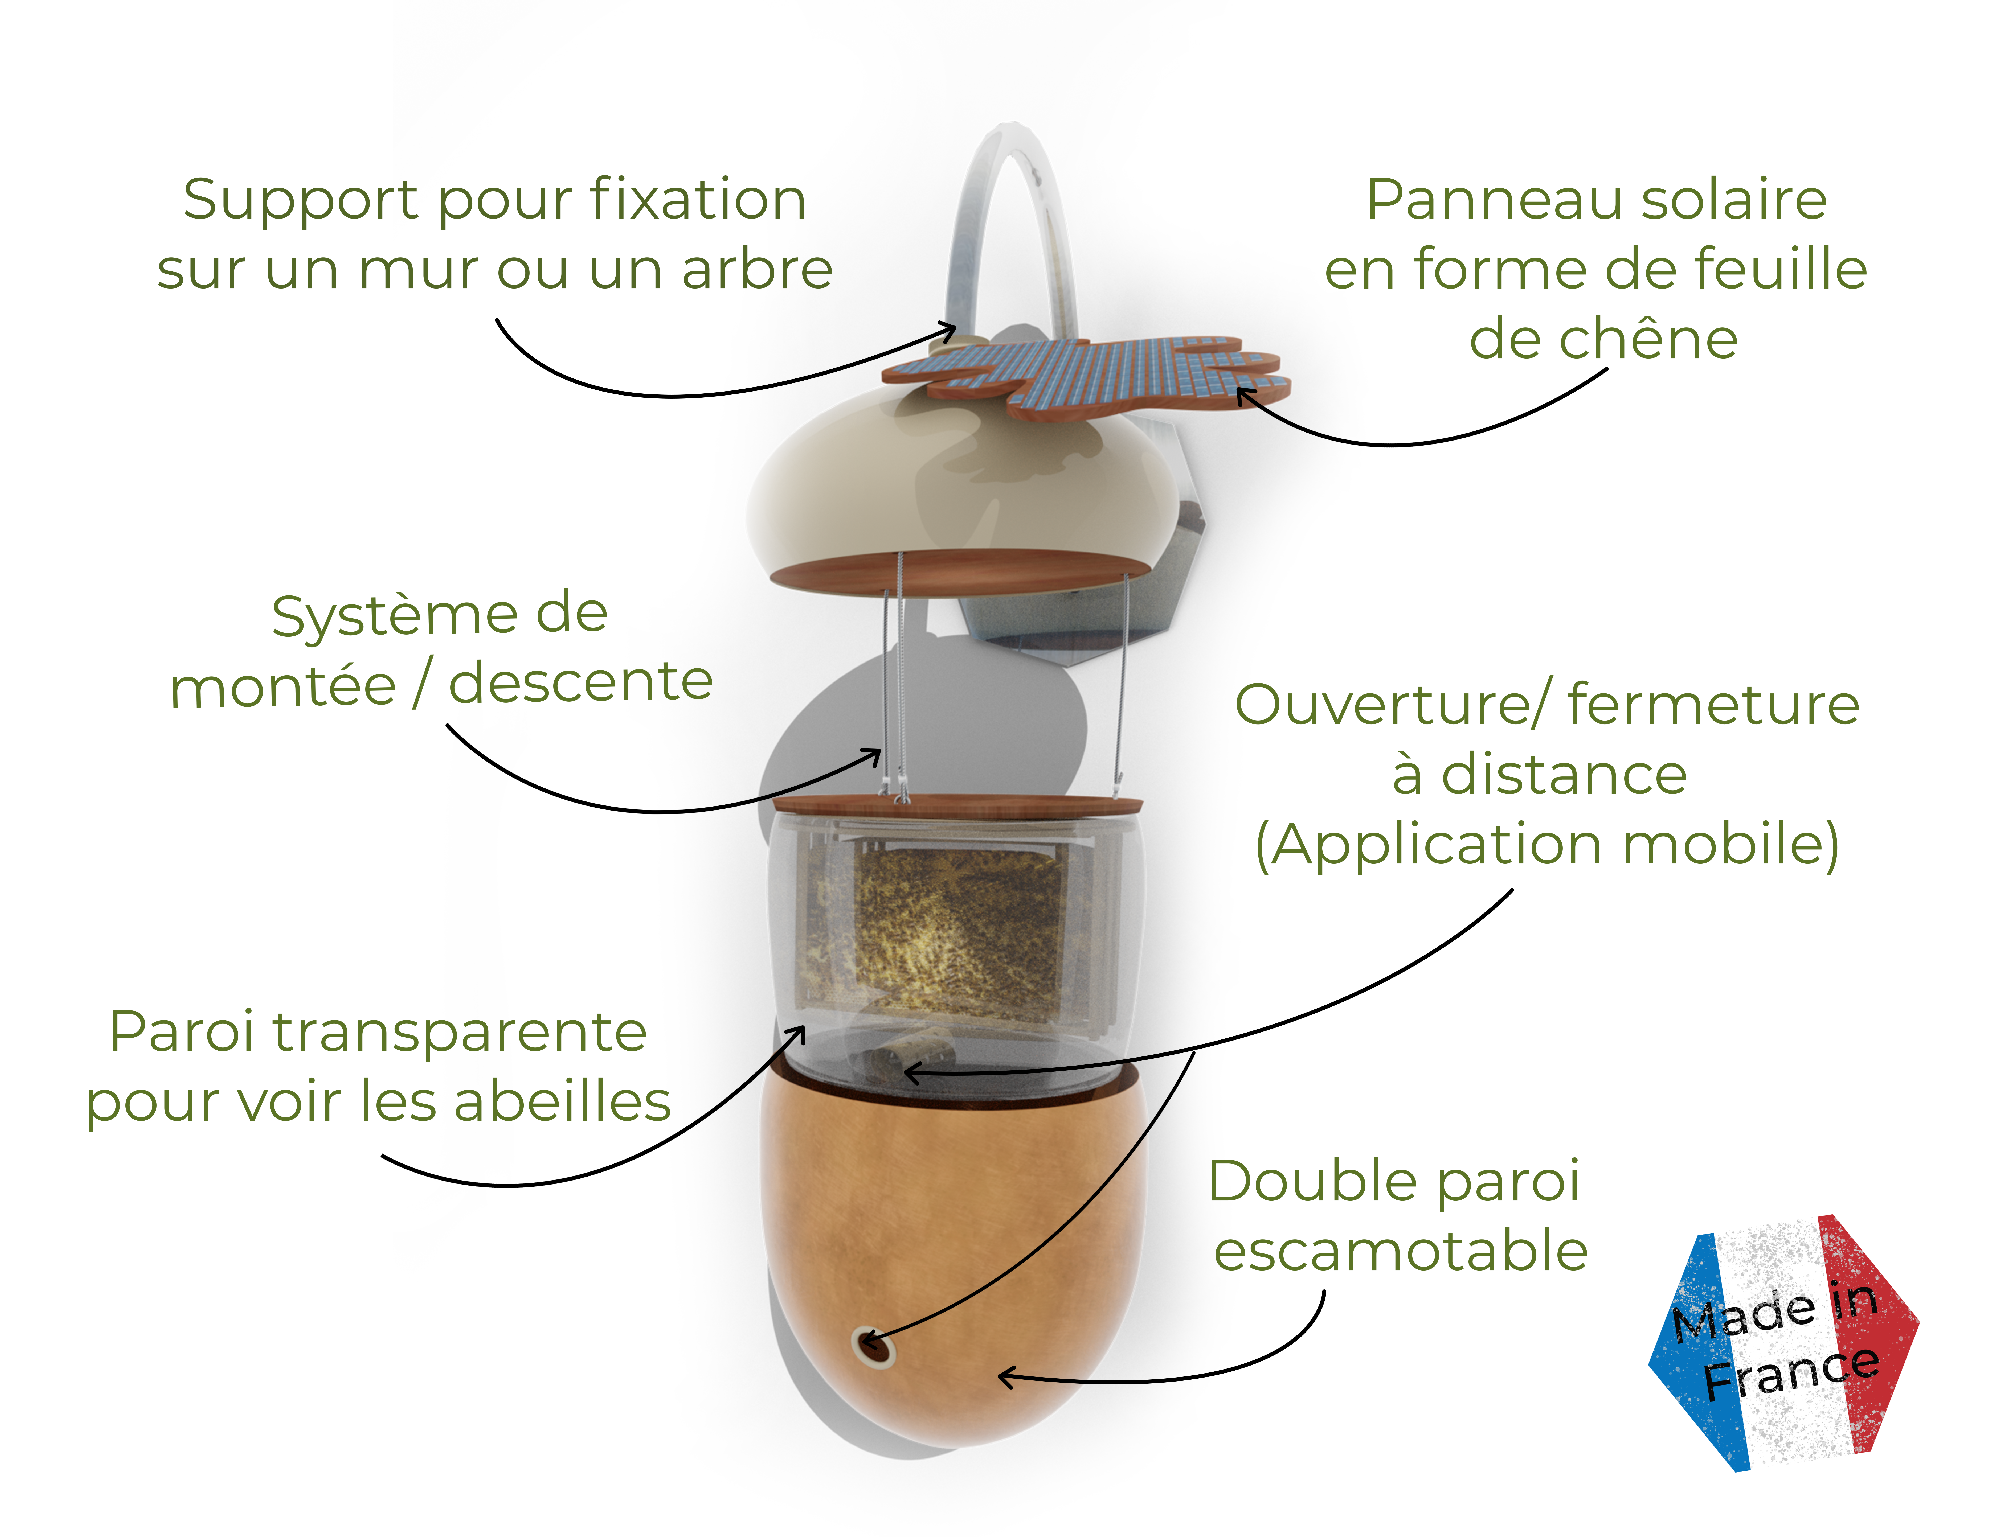
\includegraphics[width=0.4\textwidth]{Images/Simillar/rucheConnecteeOuverte.png}
		\caption{Apiago Smart Beehive \cite{Apiago}}
		\label{fig:APIAGO_HIVE}
	\end{figure}
	
	\subsubsection{HiveGenie}
	An especially advanced bee monitoring system, the HiveGenie boasts an array of 14 different sensors to remotely survey beehive activity and keep track of bee population count and flight patterns\cite{HiveGenie}. It transmits updates in intervals of 5 minutes each containing a multitude of readings giving beekeepers acute awareness of current beehive status and health. Not only does it consistently keep hive owners in the loop and but it also tracks honey flow notifying beekeepers of when they should or shouldn't feed the bees. Ultimately, the HiveGenie beehive strives to maximize honey quantity and quality while also providing both bees and beekeepers with a safe and hosptable work environment.
	\begin{figure}[H]
		\centering
		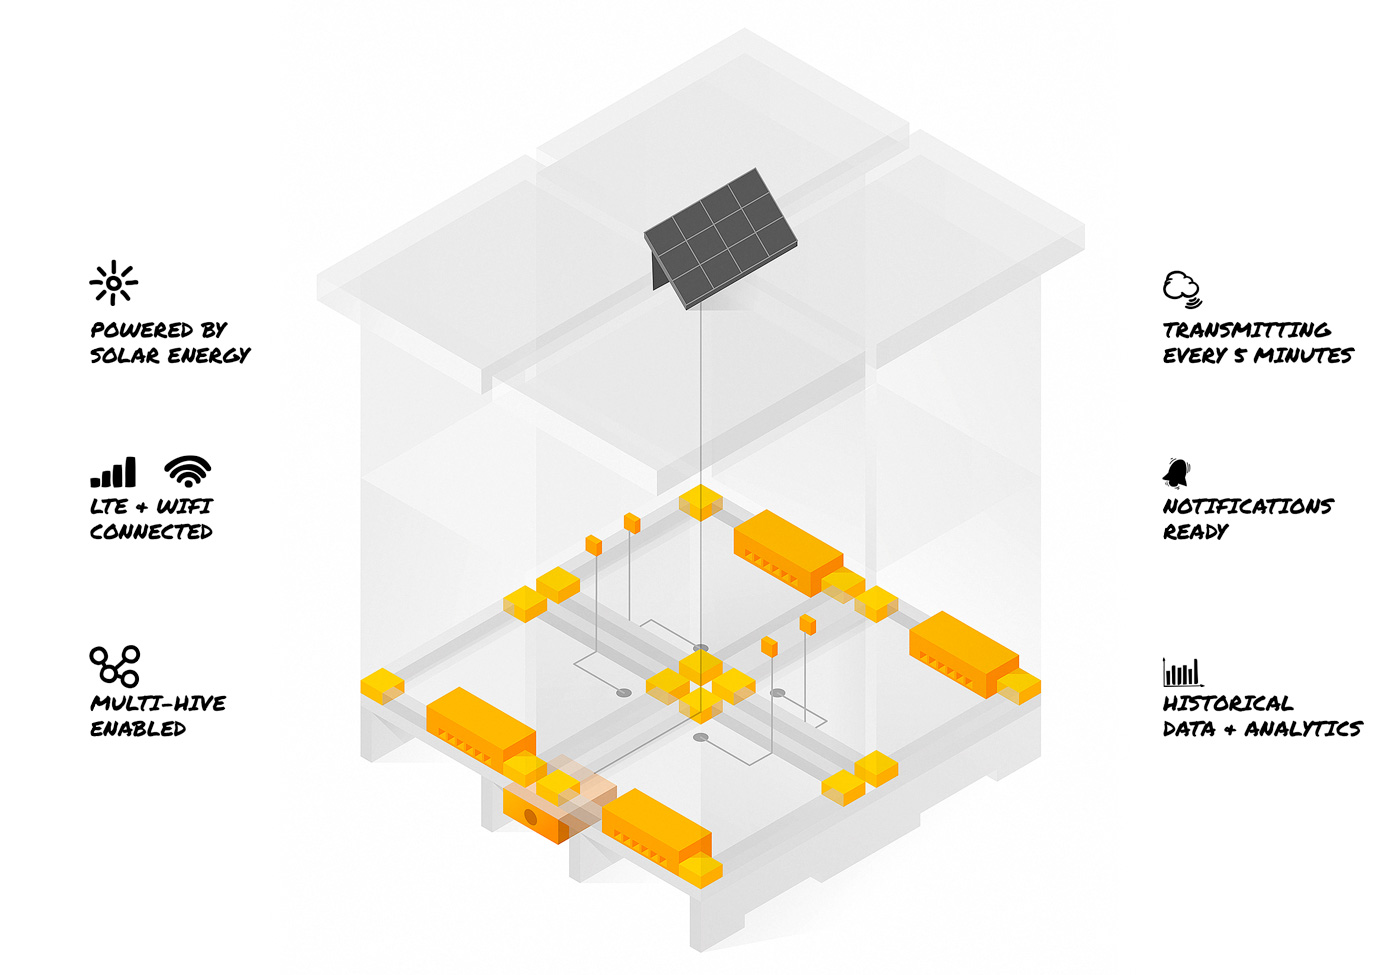
\includegraphics[width=0.4\textwidth]{Images/Simillar/hive-benefits.jpg}
		\caption{HiveGenie Beehive components \cite{HiveGenie}}
		\label{fig:HIVEGENIE_HIVE}
	\end{figure}
	
	\section{What is new in the Proposed Project?}
	The proposed Smart Beehive Monitoring System not only adds several new characteristics, but also improves features that may be found in existing hives monitoring systems. \\
	\begin{itemize}
		\item A unique innovation in the proposed system is the \textbf{cooling system} featuring an evaporative cooling pad. While prior systems have aimed to optimize hive temperature passively, the design is the first to integrate a fully functional, automated cooling system that actively stabilizes temperature and humidity within the hive. thus, conserving bees' energy while providing a more suitable and comfortable atmosphere  for them, enabling a better quality of life and ultimately contributing to a boost in their productivity. \\
		\begin{figure}[H]
			\centering
			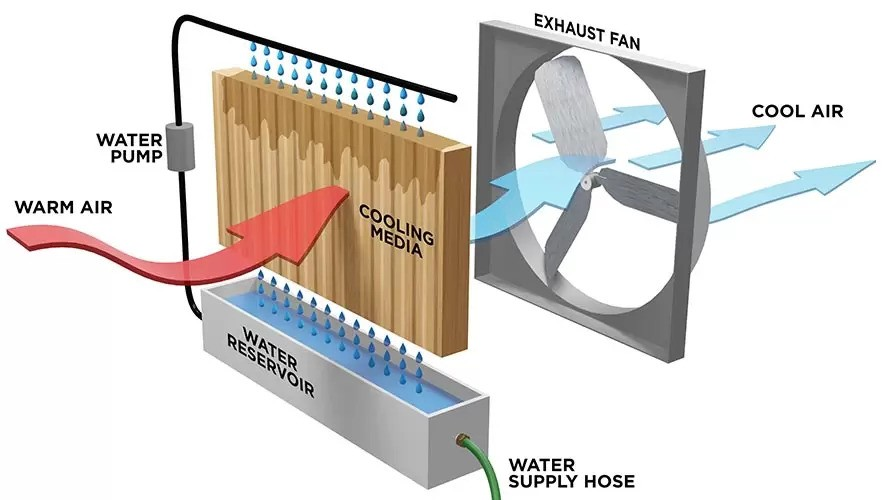
\includegraphics[width=0.5\textwidth]{Images/swamp-cooler-diagram.jpg}
			\caption{Evaporative Cooling Diagram \cite{powerbreezer2021}}
			\label{fig:EVAPORATIVE_COOLER}
		\end{figure}
		
		\item A major component of the proposed system is the \textbf{real-time recognition of bees and identification of threats} such as wasps based on visual and acoustic data provided by on door sensors. Additionally, the automated door system enables selective entry and exit of bees effectively with the inclusion of an alert system all of which enhance hive security and minimize human interference.
		\begin{figure}[H]
			\centering
			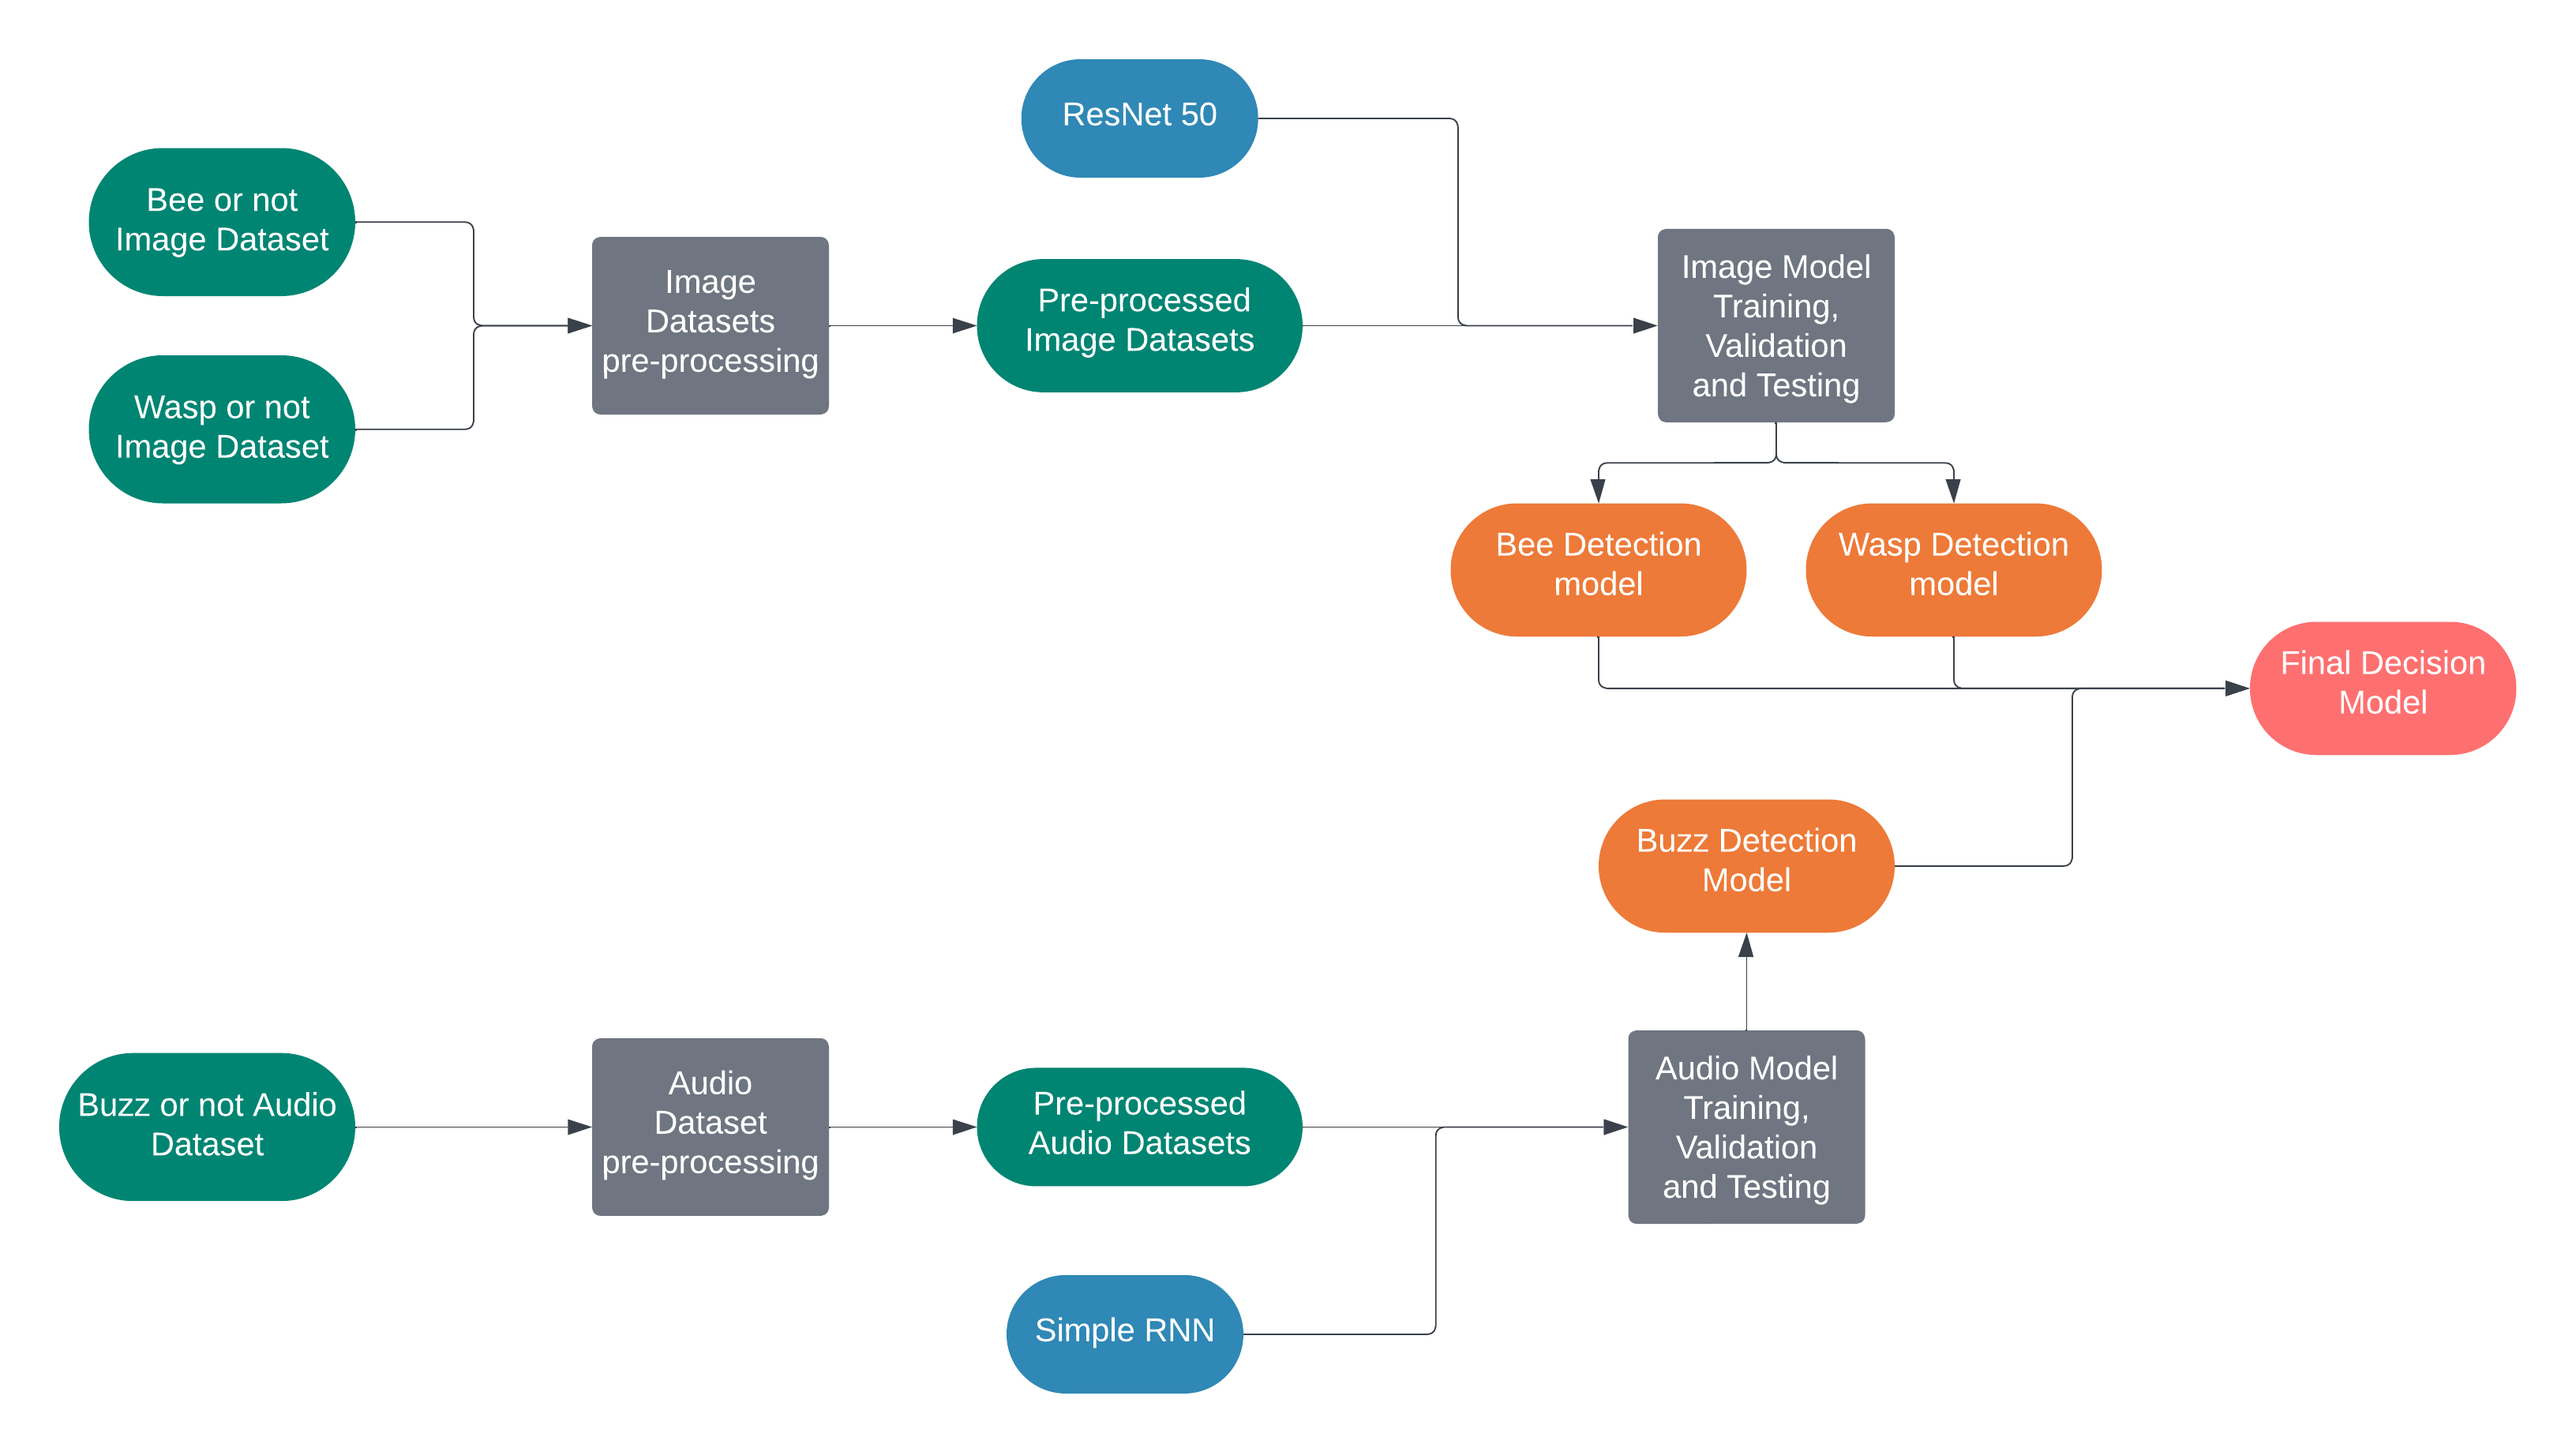
\includegraphics[width=0.9\textwidth]{Images/Pipelines/On Door Classifier Pipeline Diagram.png}
			\caption{On Door Classification}
			\label{fig:DOOR_CLASSIFICATION}
		\end{figure}
	\end{itemize}
	\newpage
	
	\section{Proof of concept}
	\subsubsection{Image based insect classification}
	Using an amalgamation of purposefully selected image datasets, which were then heavily altered using image processing techniques to attain even an even greater degree of image diversity, 6 deep learning models were put up against each other to determine the prime model to be utilized in the differentiation between bees, wasps and other insects.
	
	\begin{enumerate}
		
		\item \textbf{VGG-16} (Bee, Wasp or Other Insects) \\
		\begin{table}[H]
			\centering
			\caption{VGG Performance Metrics}
			\vspace{0.25 cm}
			\begin{tabular}{|c|c|c|c|c|}
				\hline
				\textbf{Metric} & \textbf{Bee Training} & \textbf{Bee Testing}  & \textbf{Wasp Training} & \textbf{Wasp Testing}\\
				\hline
				Accuracy & 0.8782  & 0.8968 & 0.8205  & 0.9062 \\ \hline
				Precision & 0.8727 & 0.8754  & 0.8120 & 0.9307\\ \hline
				Recall & 0.9146 & 0.9279  & 0.8521 & 0.9465 \\ \hline
				F1 Score & 0.8931 & 0.9009 & 0.8316 & 0.9385 \\ \hline
			\end{tabular}
			\label{tab:VGG_METRICS}
		\end{table}
		\begin{figure}[H]
			\centering
			\begin{minipage}{0.45\textwidth}
				\centering
				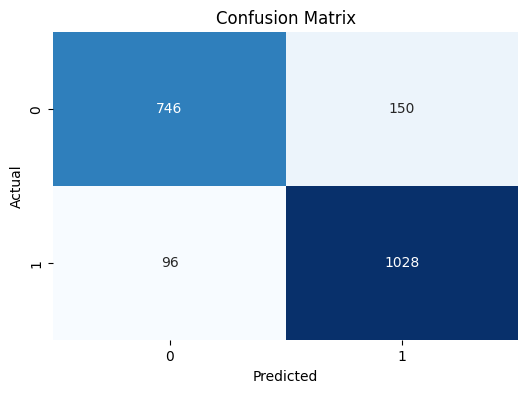
\includegraphics[width=0.8\textwidth]{Images/Confusion/vgg bees train.png}\\ \vspace{0.25 cm}
				Bee Training
			\end{minipage}
			\hfill
			\begin{minipage}{0.45\textwidth} 
				\centering           
				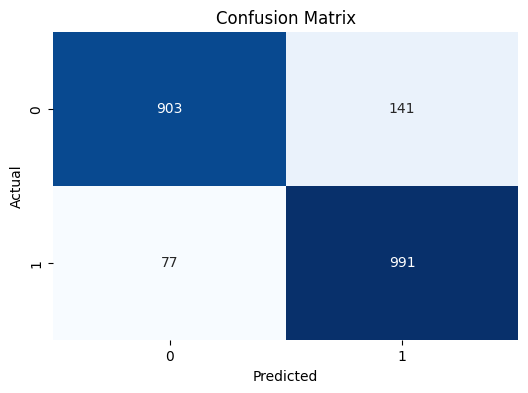
\includegraphics[width=0.8\textwidth]{Images/Confusion/vgg bees test.png} \\ \vspace{0.25 cm}
				Bee Testing
			\end{minipage}
			\newline
			\begin{minipage}{0.45\textwidth}
				\vspace{0.5 cm}
				\centering
				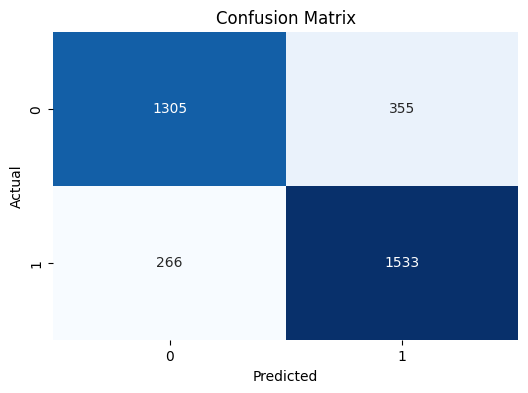
\includegraphics[width=0.8\textwidth]{Images/Confusion/vgg wasps train.png}\\ \vspace{0.25 cm}
				Wasp Training
			\end{minipage}
			\hfill
			\begin{minipage}{0.45\textwidth}
				\centering
				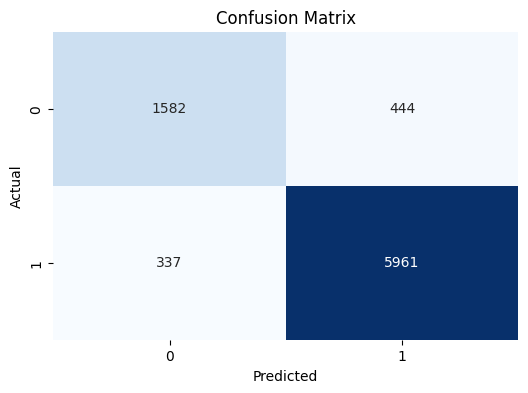
\includegraphics[width=0.8\textwidth]{Images/Confusion/vgg wasps test.png}\\ \vspace{0.25 cm}
				Wasp Testing
			\end{minipage}
			\vspace{0.5 cm}
			\caption{VGG Confusion Matrices}
		\end{figure}
		
		\item \textbf{Mobile-Net} \textit{V3 Large}  (Bee, Wasp or Other Insects) \\
		\begin{table}[H]
			\centering
			\caption{Mobile-Net Performance Metrics}
			\vspace{0.25 cm}
			\begin{tabular}{|c|c|c|c|c|}
				\hline
				\textbf{Metric} & \textbf{Bee Training} & \textbf{Bee Testing}  & \textbf{Wasp Training} & \textbf{Wasp Testing}\\
				\hline
				Accuracy & 0.8916  & 0.8987 & 0.8549  & 0.9204\\ \hline
				Precision & 0.9022 & 0.8946 & 0.8601 & 0.9411\\ \hline
				Recall & 0.9030 & 0.9064 & 0.8610 & 0.9544 \\ \hline
				F1 Score & 0.9026  & 0.9005 & 0.8606  & 0.9477 \\ \hline
			\end{tabular}
			\label{tab:MOBILE_METRICS}
		\end{table}
		\begin{figure}[H]
			\vspace{0.5 cm}
			\centering
			\begin{minipage}{0.45\textwidth}
				\centering
				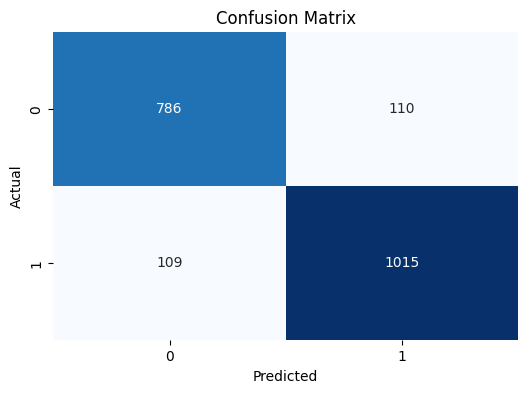
\includegraphics[width=0.8\textwidth]{Images/Confusion/mobile bees train.png} \\ \vspace{0.25 cm}
				Bee Training
			\end{minipage}
			\hfill
			\begin{minipage}{0.45\textwidth}    
				\centering
				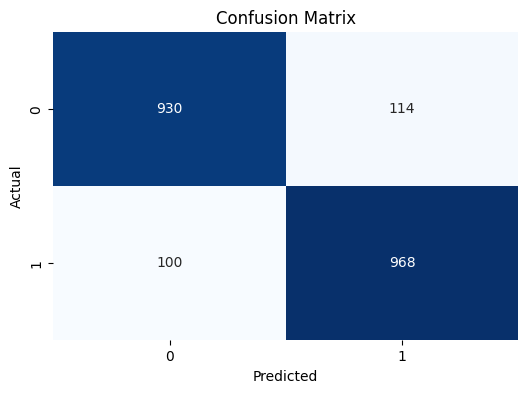
\includegraphics[width=0.8\textwidth]{Images/Confusion/mobile bees test.png} \\ \vspace{0.25 cm}
				Bee Testing
			\end{minipage}
			\newline
			\begin{minipage}{0.45\textwidth}
				\vspace{ 1.5 cm}
				\centering
				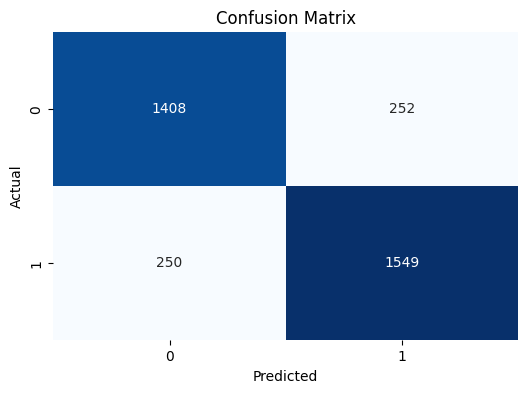
\includegraphics[width=0.8\textwidth]{Images/Confusion/mobile wasps train.png} \\ \vspace{0.25 cm}
				Wasp Training
			\end{minipage}
			\hfill
			\begin{minipage}{0.45\textwidth}
				\centering
				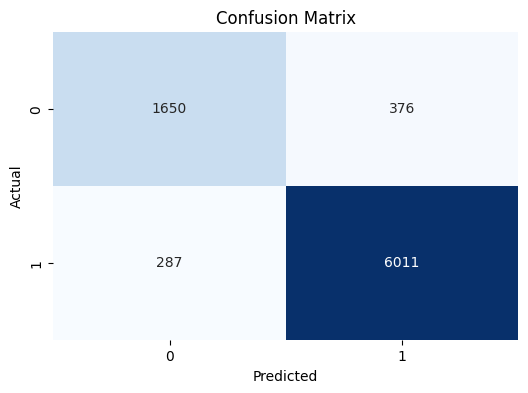
\includegraphics[width=0.8\textwidth]{Images/Confusion/mobile wasps test.png} \\ \vspace{0.25 cm}
				Wasp Testing
			\end{minipage}
			\vspace{1 cm}
			\caption{Mobile-Net Confusion Matrices}
		\end{figure}
		\newpage
		
		\item \textbf{ResNet-50} (Bee, Wasp or Other Insects) \\
		\begin{table}[H]
			\centering
			\caption{ResNet Performance Metrics}
			\vspace{0.25 cm}
			\begin{tabular}{|c|c|c|c|c|}
				\hline
				\textbf{Metric} & \textbf{Bee Training} & \textbf{Bee Testing}  & \textbf{Wasp Training} & \textbf{Wasp Testing}\\
				\hline
				Accuracy & 0.8926  & 0.8949  & 0.8624  & 0.9318  \\ \hline
				Precision & 0.8684 & 0.8591  & 0.8992 & 0.9624  \\ \hline
				Recall & 0.9511 & 0.9476 & 0.8282 & 0.9468 \\ \hline
				F1 Score & 0.9079  & 0.9012 & 0.8623  & 0.9545 \\ \hline
			\end{tabular}
			\label{tab:RESNET_METRICS}
		\end{table}
		\begin{figure}[H]
			\vspace{0.5 cm}
			\centering
			\begin{minipage}{0.45\textwidth}
				\centering
				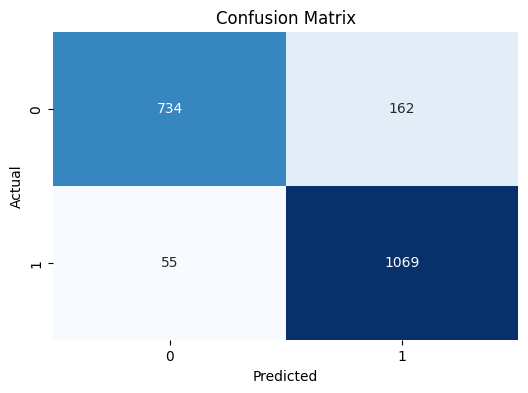
\includegraphics[width=0.8\textwidth]{Images/Confusion/res bees train.png} \\ \vspace{0.25 cm}
				Bee Training
			\end{minipage}
			\hfill
			\begin{minipage}{0.45\textwidth}    
				\centering
				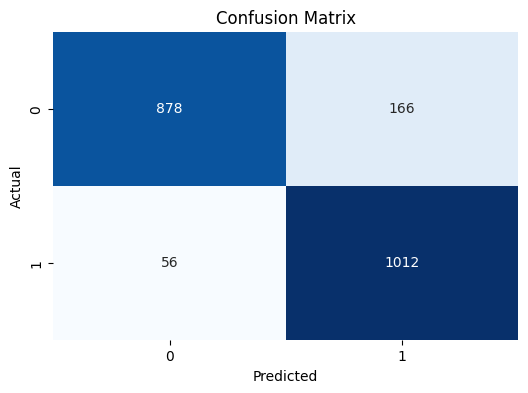
\includegraphics[width=0.8\textwidth]{Images/Confusion/res bees test.png} \\ \vspace{0.25 cm}
				Bee Testing
			\end{minipage}
			\newline
			\begin{minipage}{0.45\textwidth}
				\vspace{ 1.5 cm}
				\centering
				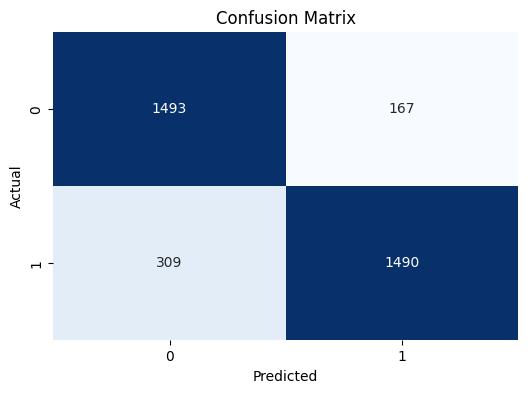
\includegraphics[width=0.8\textwidth]{Images/Confusion/res wasps train.png} \\ \vspace{0.25 cm}
				Wasp Training
			\end{minipage}
			\hfill
			\begin{minipage}{0.45\textwidth}
				\centering
				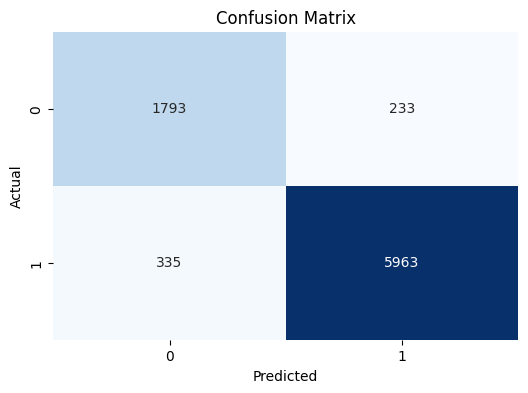
\includegraphics[width=0.8\textwidth]{Images/Confusion/res wasps test.png} \\ \vspace{0.25 cm}
				Wasp Testing
			\end{minipage}
			\vspace{1 cm}
			\caption{ResNet Confusion Matrices}
		\end{figure}
	\end{enumerate}
	As one can surmise from the previously projected metrics, it has been deduced that the optimal prime model that shall occupy the role of insect classification should be the ever-so vigilant ResNet-50 model.
	\subsubsection{Audible buzz detection}
	To aid in determining insect type, an AI audio model trained on acoustic data shall supplement the image based model in hopes of achieving better accuracies, the following are the results of the top 3 most promising candidates.
	
	\begin{enumerate}
		\item \textbf{LSTM} \\
		\begin{table}[H]
			\vspace{1 cm}
			\centering
			\caption{LSTM Performance Metrics}
			\vspace{0.25 cm}
			\begin{tabular}{|c|c|c|}
				\hline
				\textbf{Metric} & \textbf{Training} & \textbf{Testing} \\
				\hline
				Accuracy & 0.9521  & 0.9484 \\ \hline
				Precision & 0.9444 & 0.9526 \\ \hline
				Recall & 0.9590 & 0.9437 \\ \hline
				F1 Score & 0.9517  & 0.9481 \\ \hline
			\end{tabular}
			\label{tab:LSTM_METRICS}
		\end{table}
		
		\begin{figure}[H]
			\vspace{1 cm}
			\centering
			\begin{minipage}[H]{0.45\textwidth}
				\centering
				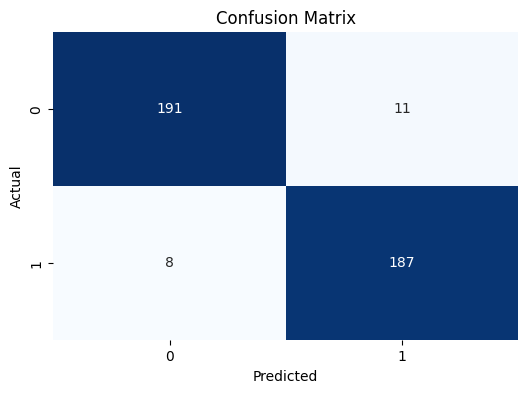
\includegraphics[width=\textwidth]{Images/Confusion/LSTM train.png}\\ \vspace{0.5 cm}
				Wasp Training
			\end{minipage}
			\hfill
			\begin{minipage}[H]{0.45\textwidth}
				\centering
				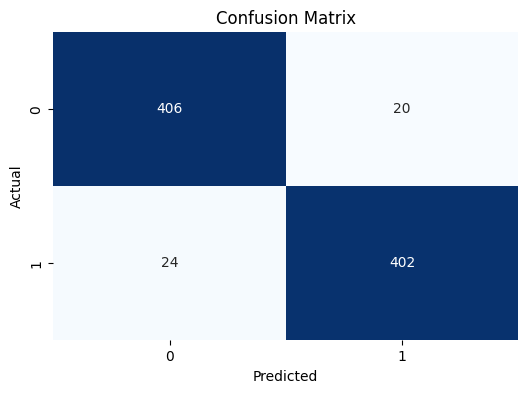
\includegraphics[width=\textwidth]{Images/Confusion/LSTM test.png}\\ \vspace{0.5 cm}
				Wasp Testing
			\end{minipage}
			\vspace{1.5 cm}
			\caption{LSTM Confusion Matrices}
		\end{figure}
		\newpage
		
		\item \textbf{GRU} \\
		\begin{table}[H]
			\centering
			\caption{GRU Performance Metrics}
			\vspace{0.25 cm}
			\begin{tabular}{|c|c|c|}
				\hline
				\textbf{Metric} & \textbf{Training} & \textbf{Testing} \\
				\hline
				Accuracy & 0.9219  & 0.8709 \\ \hline
				Precision & 0.9316 & 0.8527 \\ \hline
				Recall & 0.9077 & 0.8967 \\ \hline
				F1 Score & 0.9195  & 0.8741 \\ \hline
			\end{tabular}
			\label{tab:GRU_METRICS}
		\end{table}
		\begin{figure}[H]
			\centering
			\begin{minipage}[H]{0.45\textwidth}
				\centering
				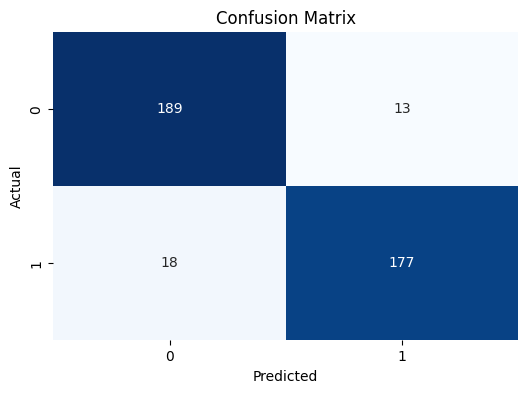
\includegraphics[width=\textwidth]{Images/Confusion/GRU train.png}\\ \vspace{0.25 cm}
				Wasp Training
			\end{minipage}
			\hfill
			\begin{minipage}[H]{0.45\textwidth}
				\centering
				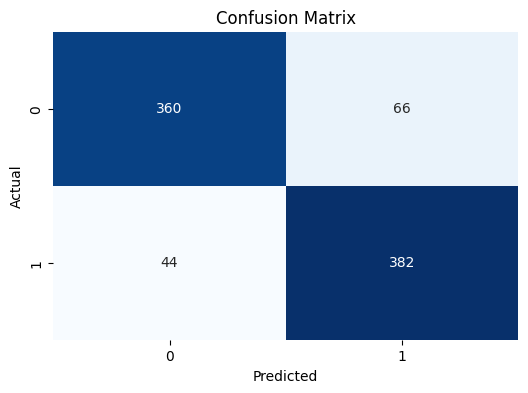
\includegraphics[width=\textwidth]{Images/Confusion/GRU test.png}\\ \vspace{0.25 cm}
				Wasp Testing
			\end{minipage}
			\vspace{1.5 cm}
			\caption{GRU Confusion Matrices}
		\end{figure}
		\item Simple RNN  \\
		
		\begin{table}[H]
			\centering
			\caption{RNN Performance Metrics}
			\vspace{0.25 cm}
			\begin{tabular}{|c|c|c|}
				\hline
				\textbf{Metric} & \textbf{Training} & \textbf{Testing} \\
				\hline
				Accuracy & 0.9572  & 0.9695 \\ \hline
				Precision & 0.9588 & 0.9717 \\ \hline
				Recall & 0.9538 & 0.9671 \\ \hline
				F1 Score & 0.9563  & 0.9694 \\ \hline
			\end{tabular}
			\label{tab:RNN_METRICS}
		\end{table}
		\begin{figure}[H]
			\centering
			\begin{minipage}[H]{0.45\textwidth}
				\centering
				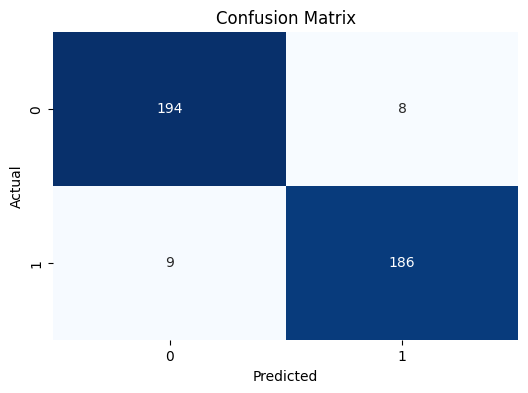
\includegraphics[width=\textwidth]{Images/Confusion/RNN train.png}\\ \vspace{0.5 cm}
				Wasp Training
			\end{minipage}
			\hfill
			\begin{minipage}[H]{0.45\textwidth}
				\centering
				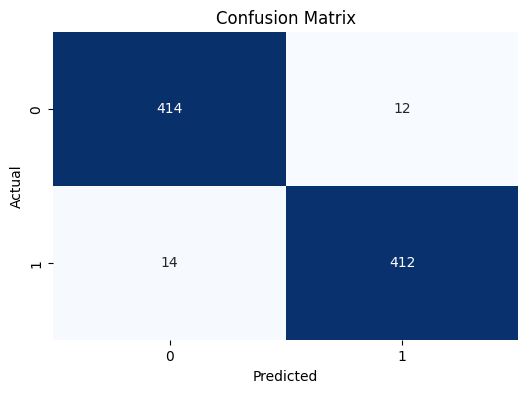
\includegraphics[width=\textwidth]{Images/Confusion/RNN test.png}\\ \vspace{0.5 cm}
				Wasp Testing
			\end{minipage}
			\vspace{1.5 cm}
			\caption{RNN Confusion Matrices}
		\end{figure}
	\end{enumerate} 
	Upon close inspection of the formerly disclosed results, it was settled that the Simple RNN model would be the superior model that shall shoulder the burden of detecting insect buzzing sounds.
	
	\subsection{Temperature and Humidity Forecasting}
	\begin{itemize}
		
		\item Among the forecasting process, five different forecasting models were utilized to evaluate the best-performing one based on a set of accuracy metrics. The table below shows the performance of each model along with their metrics, including MASE, RMSSE, MAE, RMSE, MAPE, and SMAPE.
		
		\begin{table}[H]
			\caption{Performance Metrics for Forecasting Models}
			\label{tab:FORECAST_METRICS}
			\vspace{0.25 cm}
			\resizebox{\columnwidth}{!}{%
				\begin{tabular}{|l|c|c|c|c|c|c|}
					\hline
					\textbf{Model} & \textbf{MASE} & \textbf{RMSSE} & \textbf{MAE} & \textbf{RMSE} & \textbf{MAPE} & \textbf{SMAPE} \\ \hline
					ARIMA & 0.0486 & 0.0400 & 0.0112 & 0.0112 & 0.0008 & 0.0008 \\ \hline
					Naive Forecaster & 0.4943 & 0.4064 & 0.1142 & 0.1142 & 0.0077 & 0.0076 \\ \hline
					Extra Trees w/ Cond. Deseasonalize & 0.6543 & 0.5375 & 0.1505 & 0.1505 & 0.0102 & 0.0100 \\ \hline
					Grand Means Forecaster & 0.7575 & 0.6228 & 0.1751 & 0.1751 & 0.0117 & 0.0118 \\ \hline
					Croston & 0.8001 & 0.6576 & 0.1844 & 0.1844 & 0.0124 & 0.0123 \\ \hline
				\end{tabular}%
			}
		\end{table}
		
		
		From this observation, the \textbf{ARIMA} model outperformed the highest accuracy with the lowest error across all metrics. Hence, we decided to select ARIMA to proceed with further analysis for forecasting in both temperature and humidity.
		
		
		\item{Hardware Trigger Pseudo-Code}
		
		The mentioned pseudo-code summarizes the implementation we used of the hardware trigger for temperature and humidity monitoring:
		
		\begin{verbatim}
			1. Initialize DHT sensor and LED pin
			2. Set initial humidity threshold to 60.0%
			3. Start loop:
			a. If new threshold received from Serial input:
			- Update humidity threshold
			b. Read current humidity and temperature
			c. If reading is valid:
			- Display humidity and temperature
			- If humidity exceeds threshold:
			* Turn on LED
			- Else:
			* Turn off LED
			d. If reading fails:
			- Print error message
			- Ensure LED is off
			e. Wait for 1 second before next reading
		\end{verbatim}
		
		\begin{figure}[H]
			\centering
			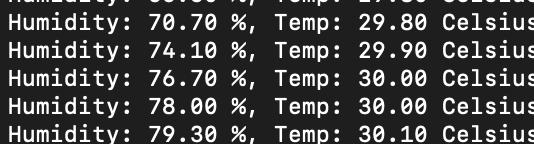
\includegraphics[width=0.5\textwidth]{Images/Test/WhatsApp Image 2024-11-11 at 19.50.57_53e5664d.jpg}
			\caption{Sensor Readings}
		\end{figure}
		
		\begin{itemize}
			\item Having started testing the implementation of a hardware trigger based on the chosen model, a simulation of the alert system is initiated when a threshold, as determined by the model is reached. \\
			
			\begin{minipage}[H]{0.45\textwidth}
				\begin{figure}[H]
					
					\centering
					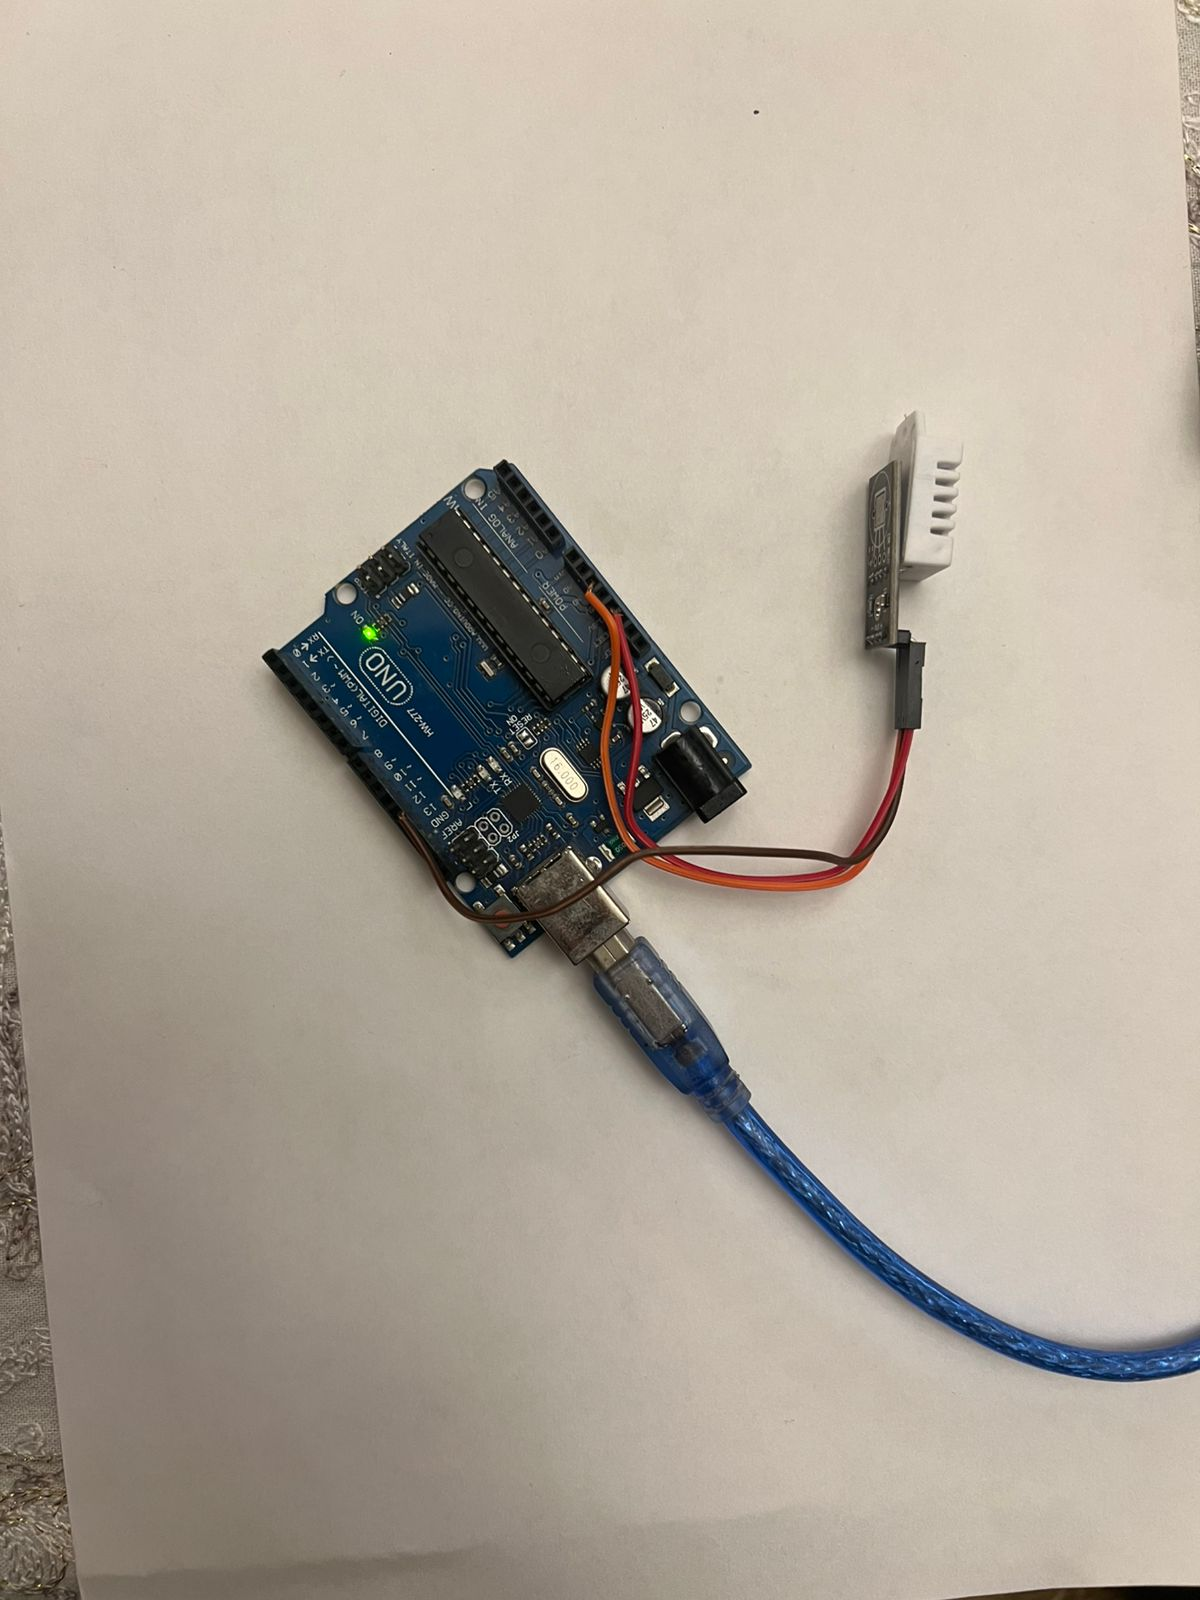
\includegraphics[width=0.7\textwidth]{ Images/Test/WhatsApp Image 2024-11-11 at 19.50.24_cb32c8b9.jpg}
					\caption{Normal State}
				\end{figure}
			\end{minipage}
			\hfill
			\begin{minipage}[H]{0.45\textwidth}
				\begin{figure}[H]
					\centering
					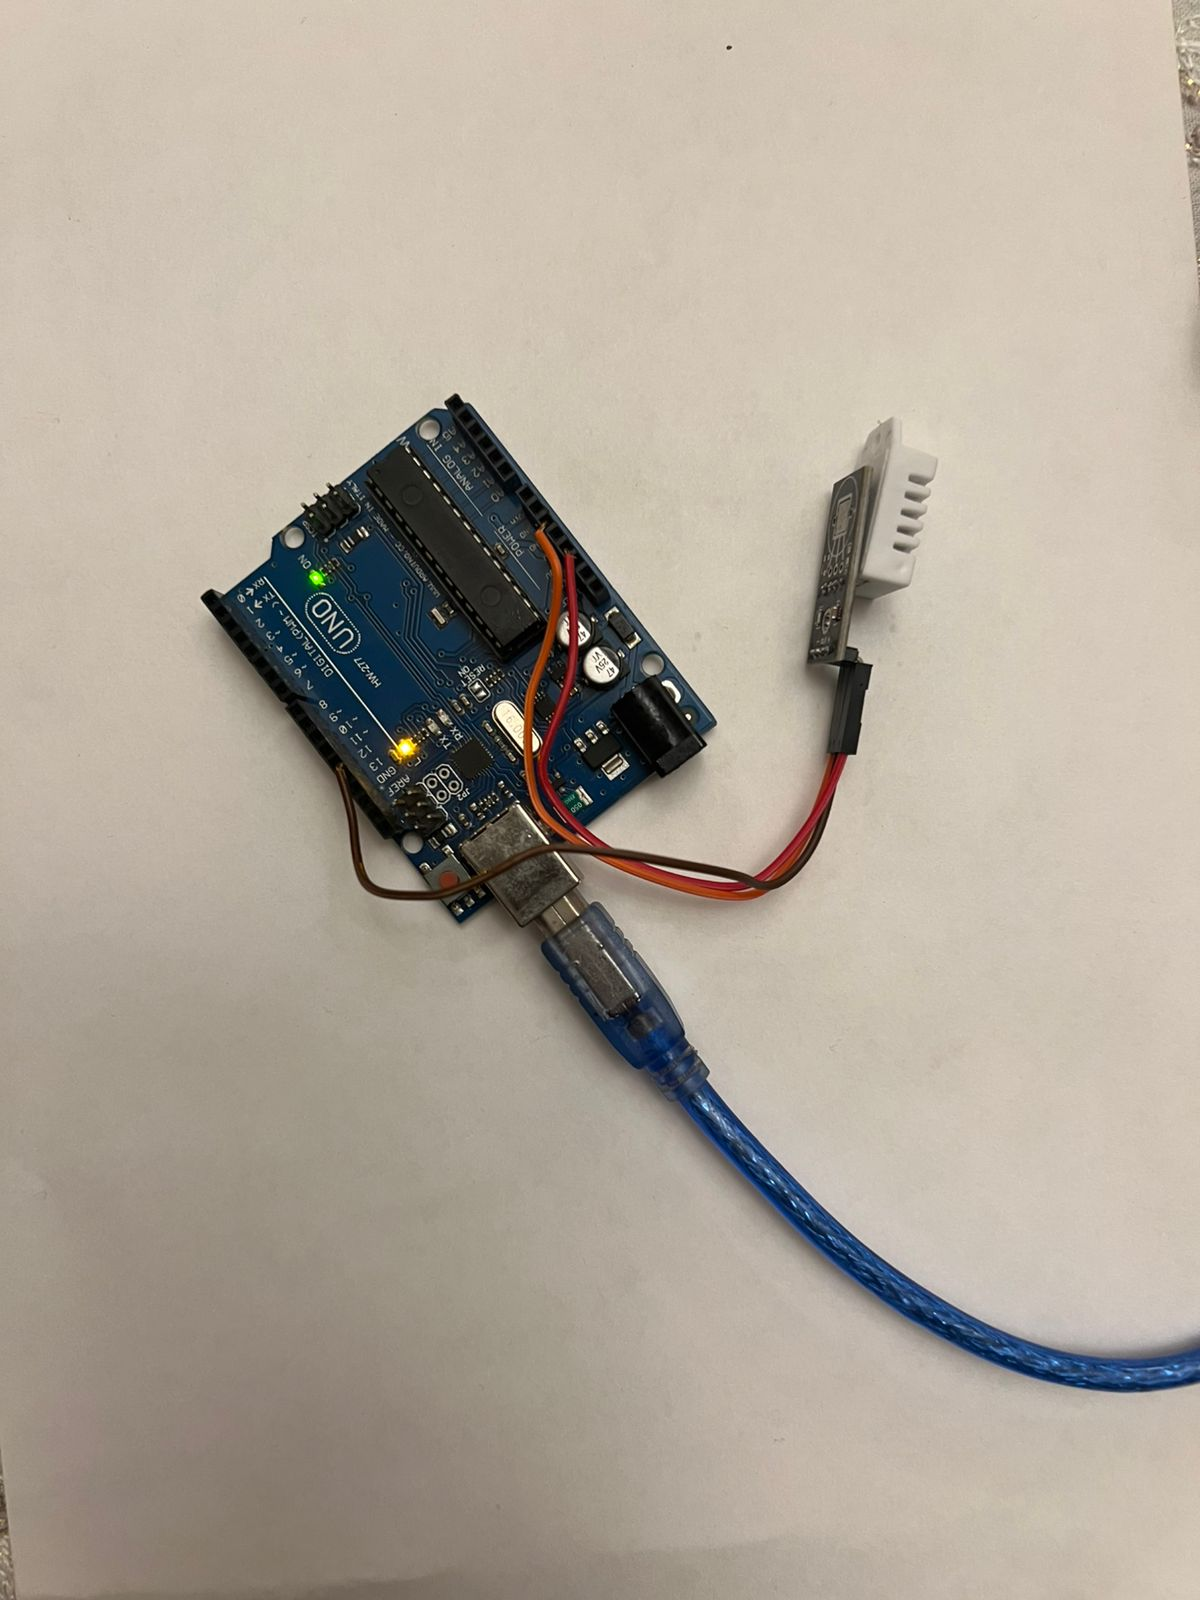
\includegraphics[width=0.7\textwidth]{Images/Test/WhatsApp Image 2024-11-11 at 19.50.24_5aa74f64.jpg}
					\caption{Threshold Triggered the Light On}
				\end{figure}
			\end{minipage}
		\end{itemize}
	\end{itemize}
	\newpage
	\section{Project Management and Deliverables}
	\subsection{Deliverables}
	The expected project deliverables shall be submitted for arbitration and review on a per milestone basis as illustrated in the diagram below: 
	\vspace{0.5 cm}
	\begin{figure}[H]
		\centering
		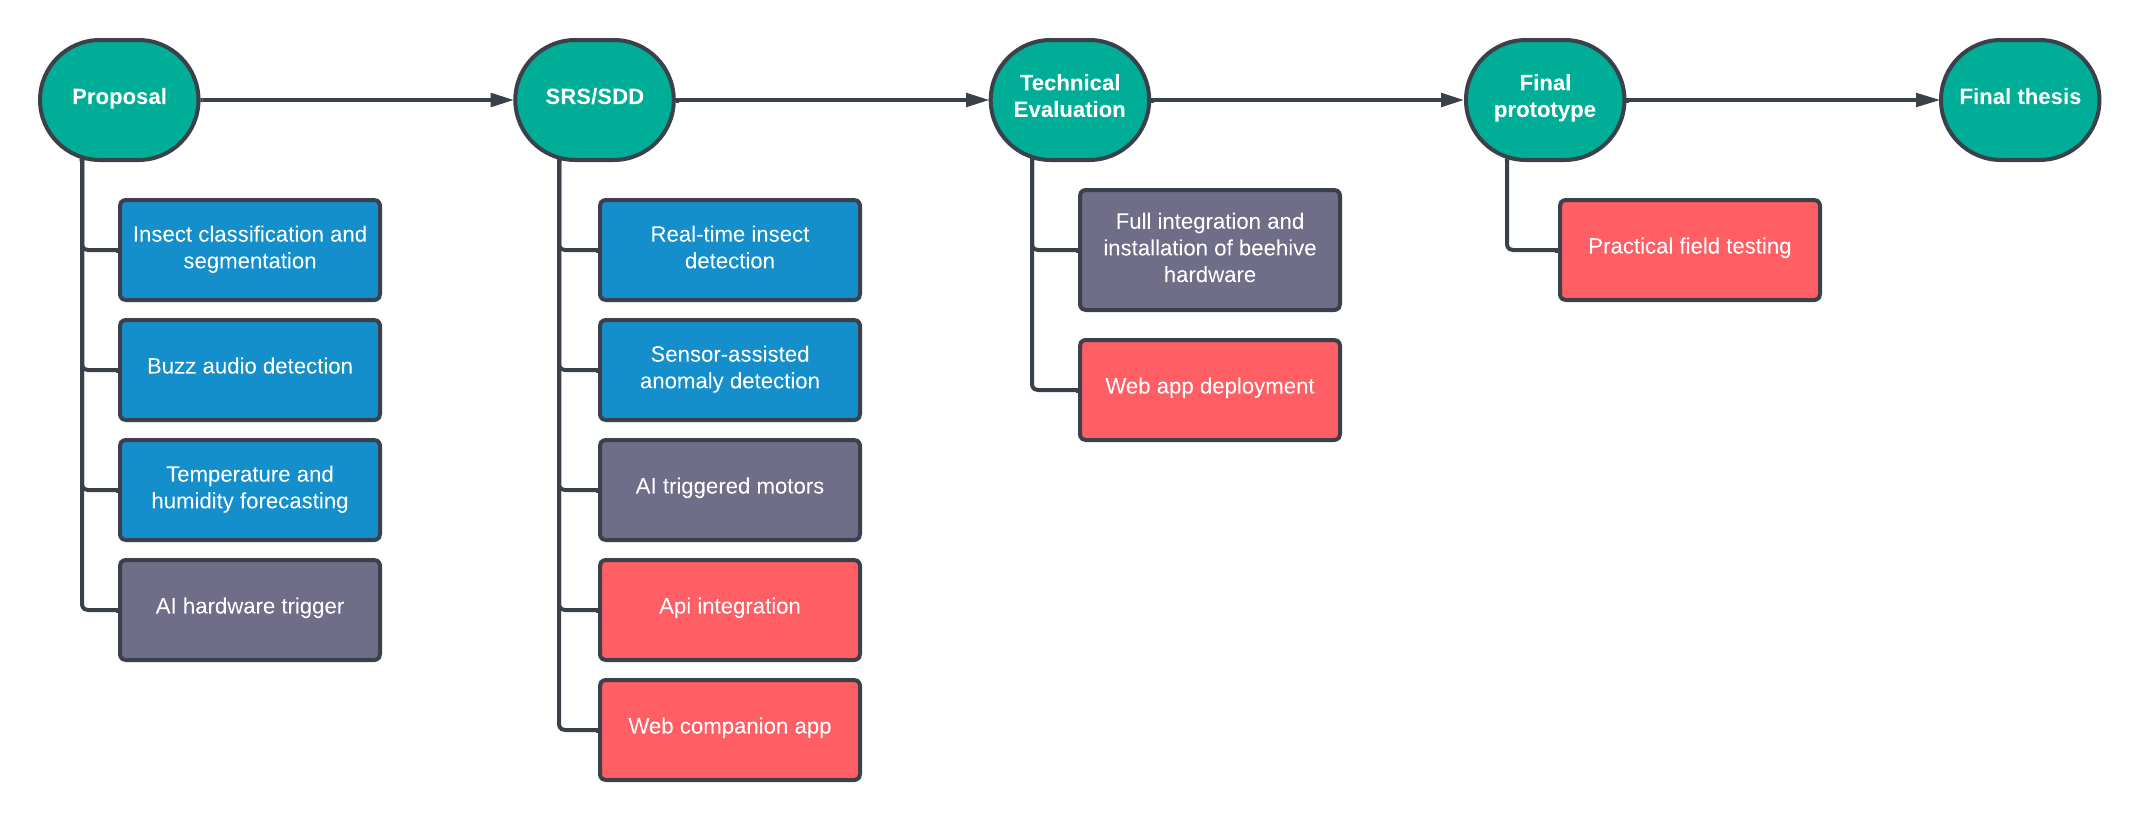
\includegraphics[width=\textwidth]{Images/Pipelines/Mele-Deliverables.png}
		\caption{Project Deliverables}
		\label{fig:DELIVERABLES}
	\end{figure}
	
	\vspace{1 cm}
 \begin{table}[H]
	\centering
	\caption{Project Deliverables Brief}
	\vspace{0.25 cm}
	\resizebox{\textwidth}{!}{%
		\begin{tabular}{|>{\centering\arraybackslash}m{5 cm}|m{5 cm}|m{5 cm}|m{5 cm}|}
			\hline
			\textbf{Milestones} & \textbf{AI Models} & \textbf{Hardware implementation} & \textbf{Miscellaneous} \\ \hline
			\begin{enumerate}
				\item Proposal
				\item SRS and SDD
				\item Technical evaluation
				\item Final prototype
				\item Final thesis
			\end{enumerate}
			&\begin{enumerate}
				\item Insect classification and segmentation
				\item Buzz audio detection
				\item Temperature and humidity forecasting
				\item Real-time insect detection
				\item Sensor-assisted anomaly detection
			\end{enumerate}
			&\begin{enumerate}
				\item AI hardware trigger
				\item AI triggered motors
				\item Full integration and installation of beehive hardware
			\end{enumerate}
			&\begin{enumerate}
				\item API integration
				\item Web companion app
				\item Web app deployment
				\item Practical field testing
			\end{enumerate}
			\\ \hline
			
		\end{tabular}%
	}
\end{table}
	\vspace{1 cm} \hspace{-0.78 cm}
	Having laid out the awaited outputs of the project in such a simple and concise manner, it is the team's aspiration to not only commit to consistently achieving said targets but to also do so in a timely fashion.
	\newpage
	\subsection{Tasks and Time Plan}
	\vspace{ 1 cm}
	\begin{figure}[H]
		\centering
		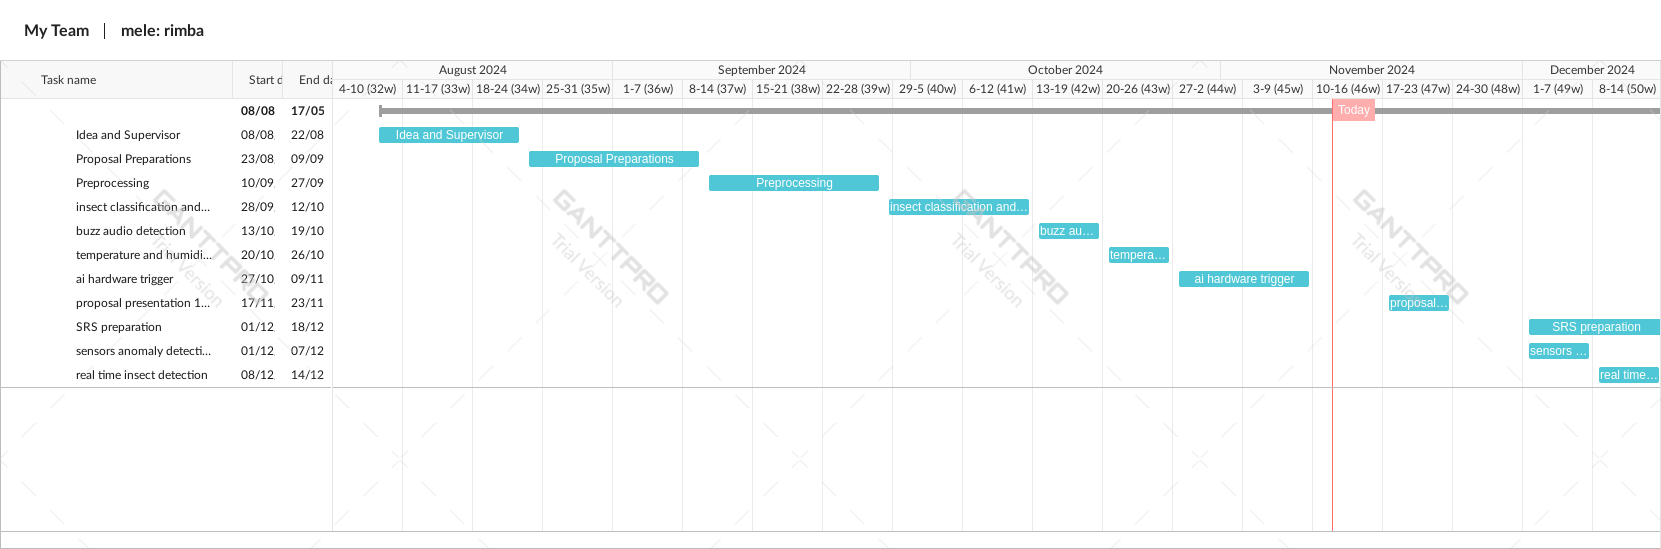
\includegraphics[width=\textwidth]{Images/Management/mele1.png}
	\end{figure}
	\begin{figure}[H]
		\centering
		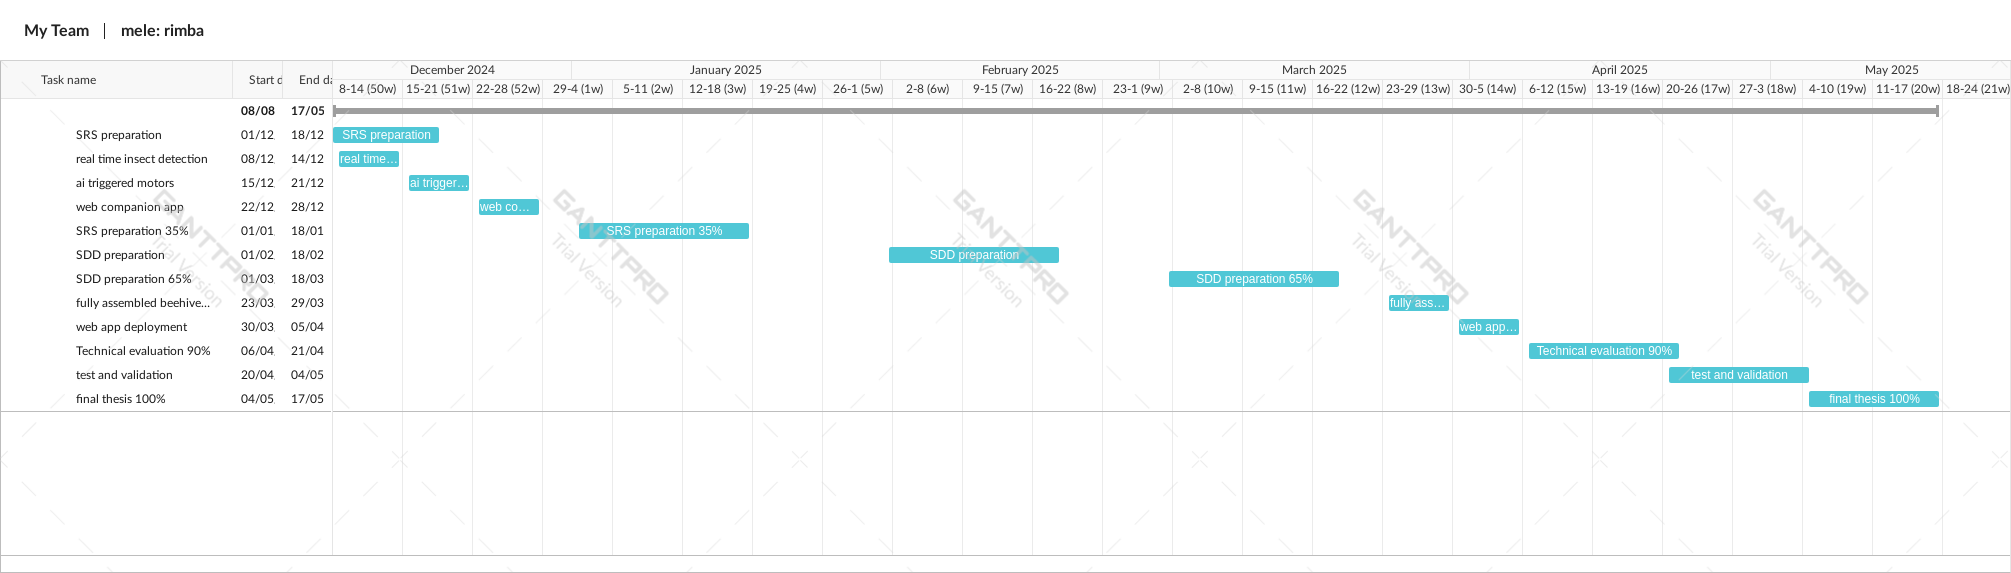
\includegraphics[width=\textwidth]{Images/Management/mele2.png}
		\label{fig:CHART}
		\caption{Task and Time Management Plan}
	\end{figure}
	\vspace{2 cm}
	This Diagram is made by \textbf{GanttPro \cite{ganttpro}} to map the project's timeline with its tasks and deliverables, to ensure the provision of a well-maintained workflow and a timely road-map of the project's progress. In other words, having an organized reference and visualization of the project's milestones and deadlines, alongside all of its phases, facilitates progress tracking and allows for any schedule adjustments needed to meet the project's goals.
	\newpage
	\subsection{Budget and Resource Costs}
	It goes without saying, all the advancements introduced and suggested to the typical and conventional beehive structure would require the installation of numerous components. All the prices listed below were collected from an electronics store called \textbf{Future Electronics} \cite{fut_electronics}located in Cairo, Egypt. \\ \newline
	Notably, all these calculations are merely rough estimations of the expected production range, excluding the cost of the sustaible power supply, \textit{the solar grid}, and its operating battery, as well as the cost of the actual wood work required to build any hive.
	\vspace{0.5 cm}
	\begin{figure}[H]
		\centering
		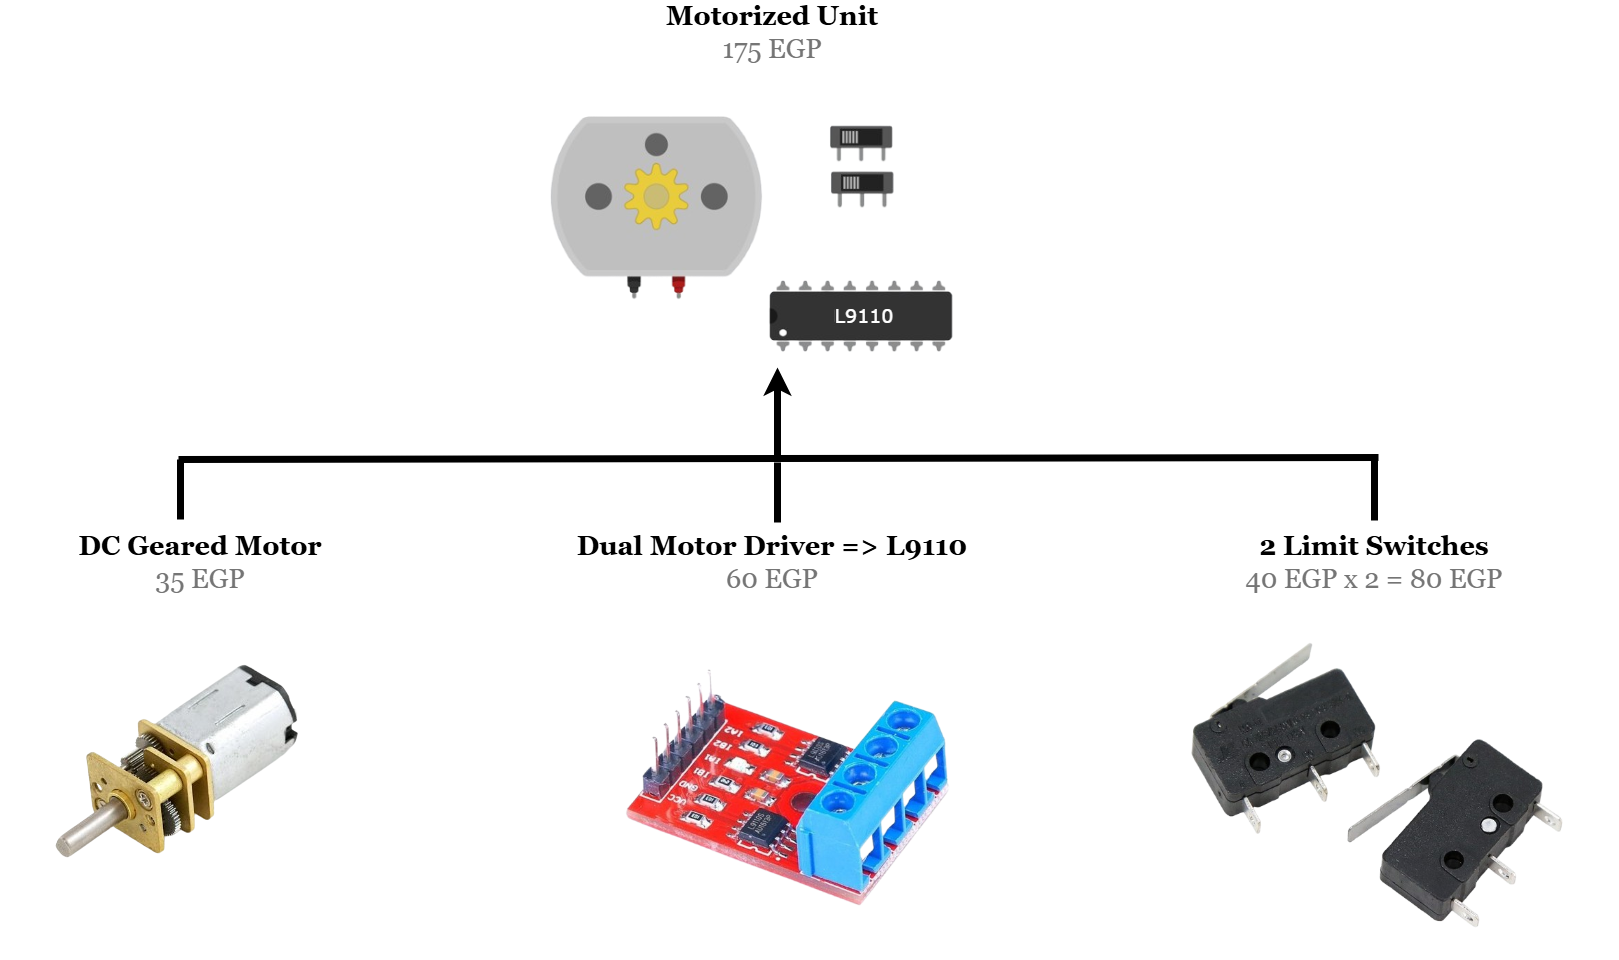
\includegraphics[width=0.6\textwidth]{Images/Components/Motorized Unit Cost.png}
		\caption{Motorized Unit Cost }
		\label{fig:MOTORIZED_COST}
	\end{figure}
	\vspace{0.5 cm}
	\begin{figure}[H]
		\centering
		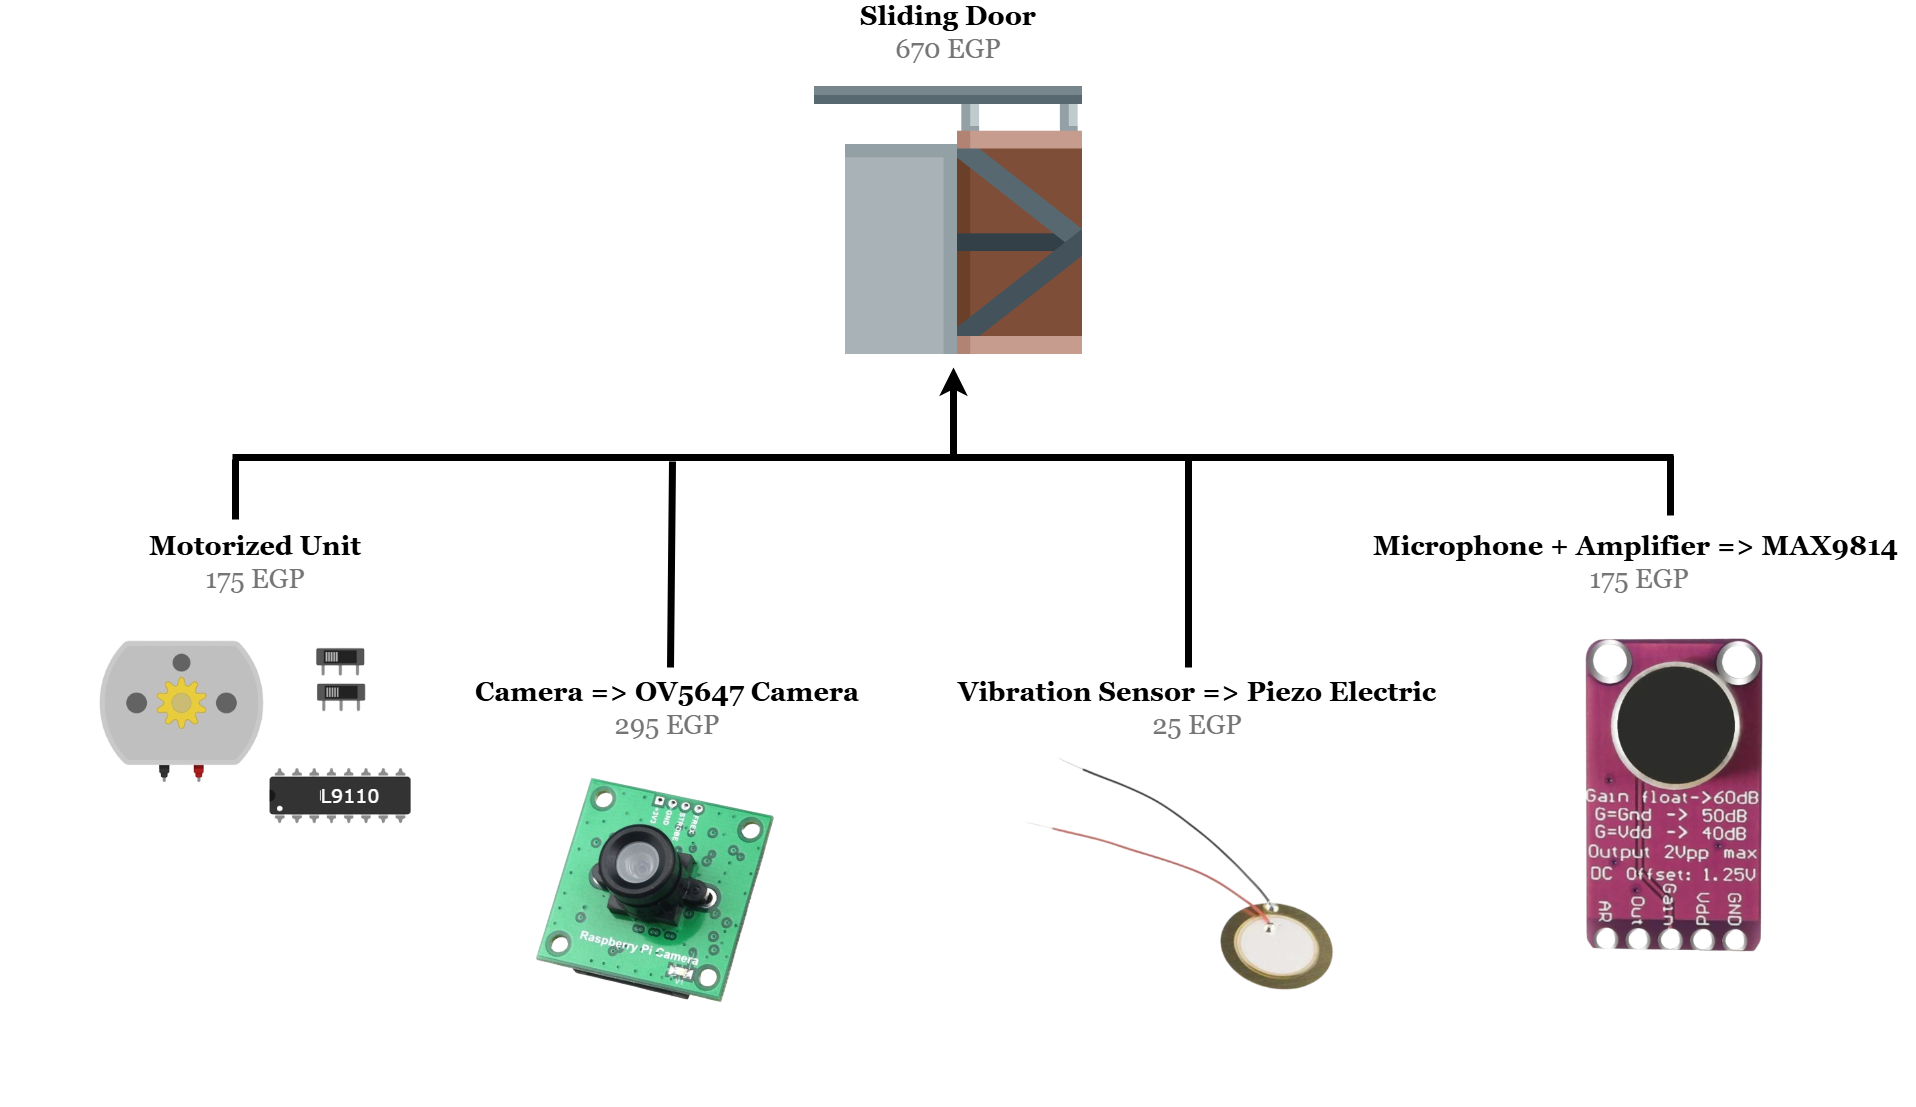
\includegraphics[width=0.7\textwidth]{Images/Components/Sliding Door Cost.png}
		\caption{Sliding Door Cost }
		\label{fig:DOOR_COST}
	\end{figure}
	\begin{figure}[H]
		\centering
		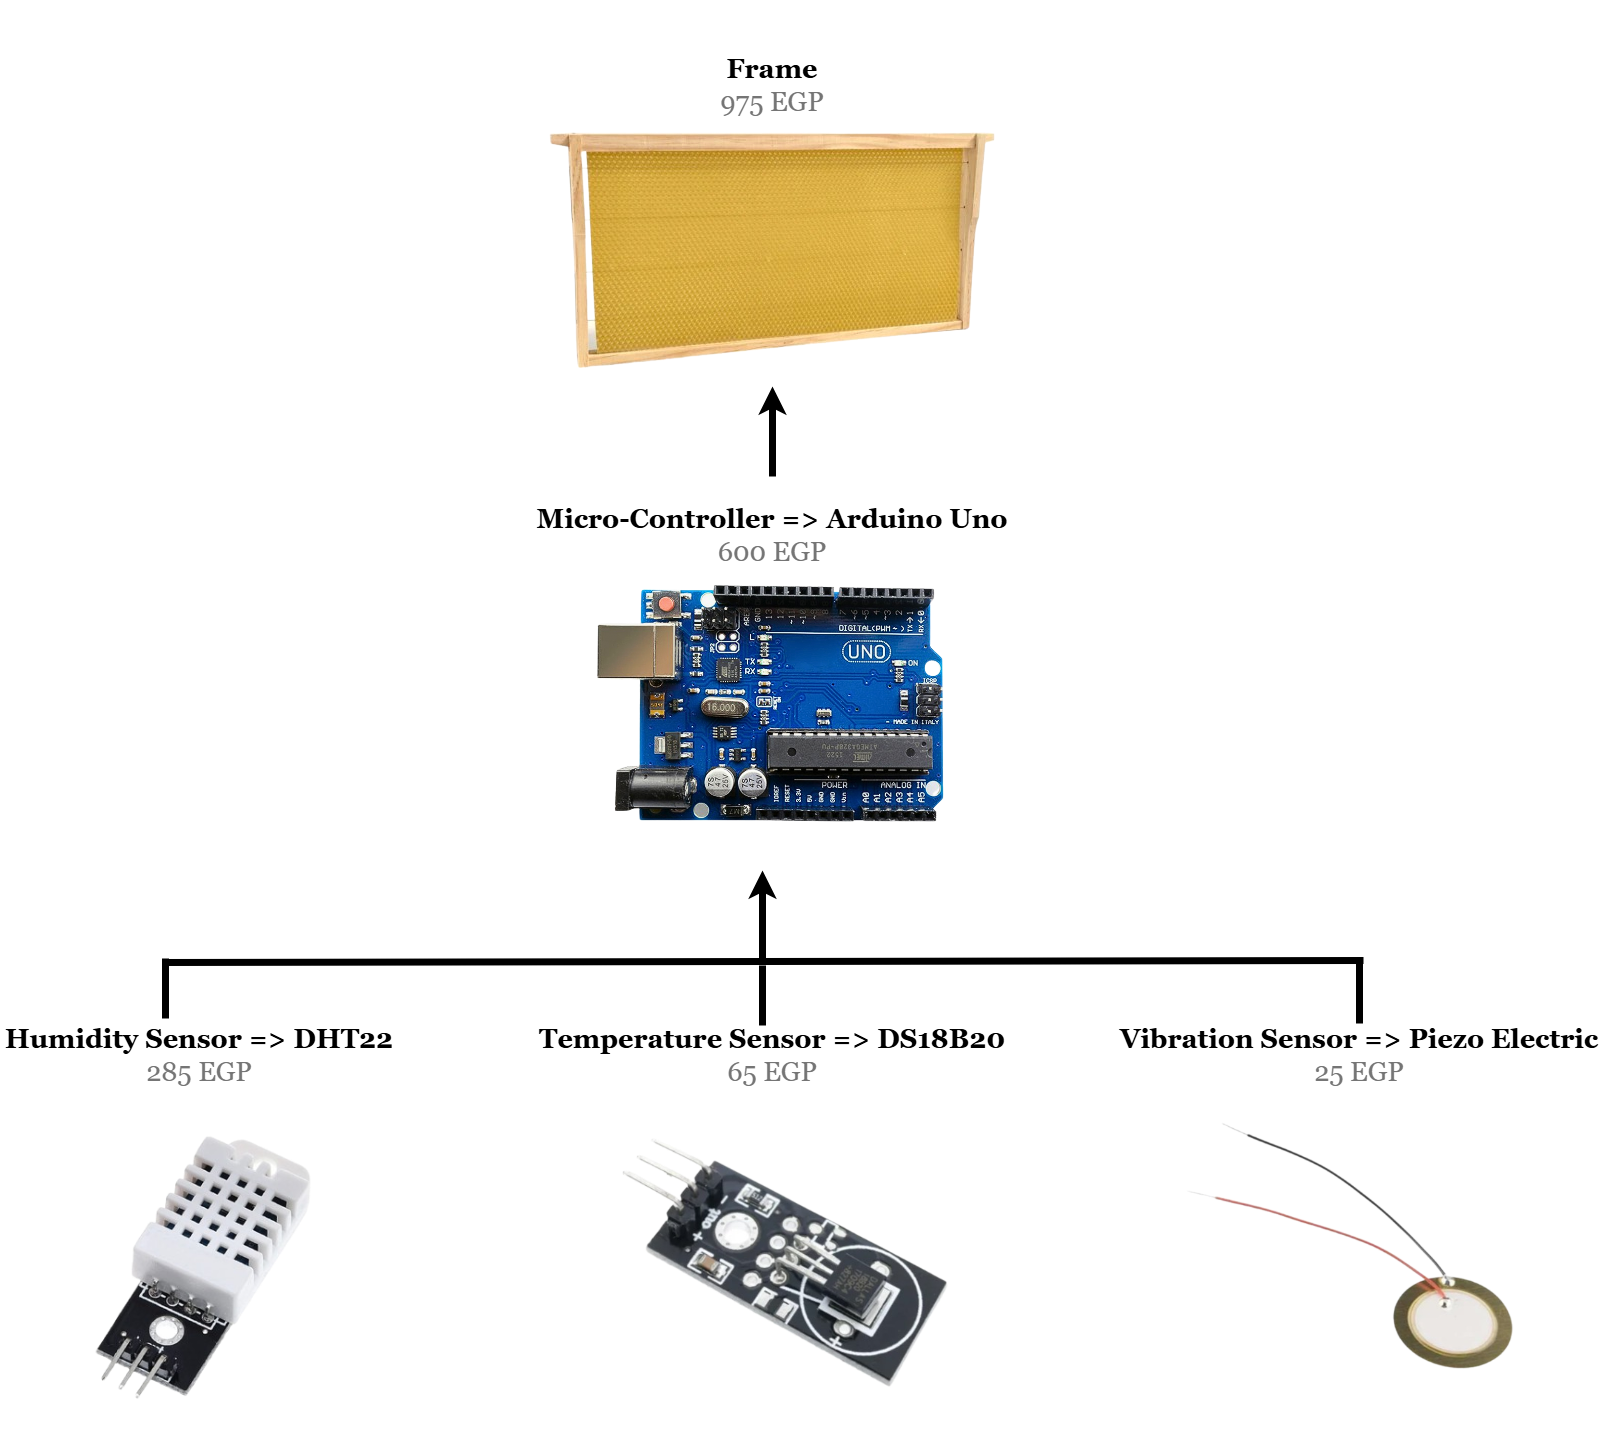
\includegraphics[width=0.8\textwidth]{Images/Components/Frame Cost.png}
		\caption{Sensor Frame Cost }
		\label{fig:FRAME_COST}
	\end{figure}
	\vspace{0.3 cm}
	\begin{figure}[H]
		\centering
		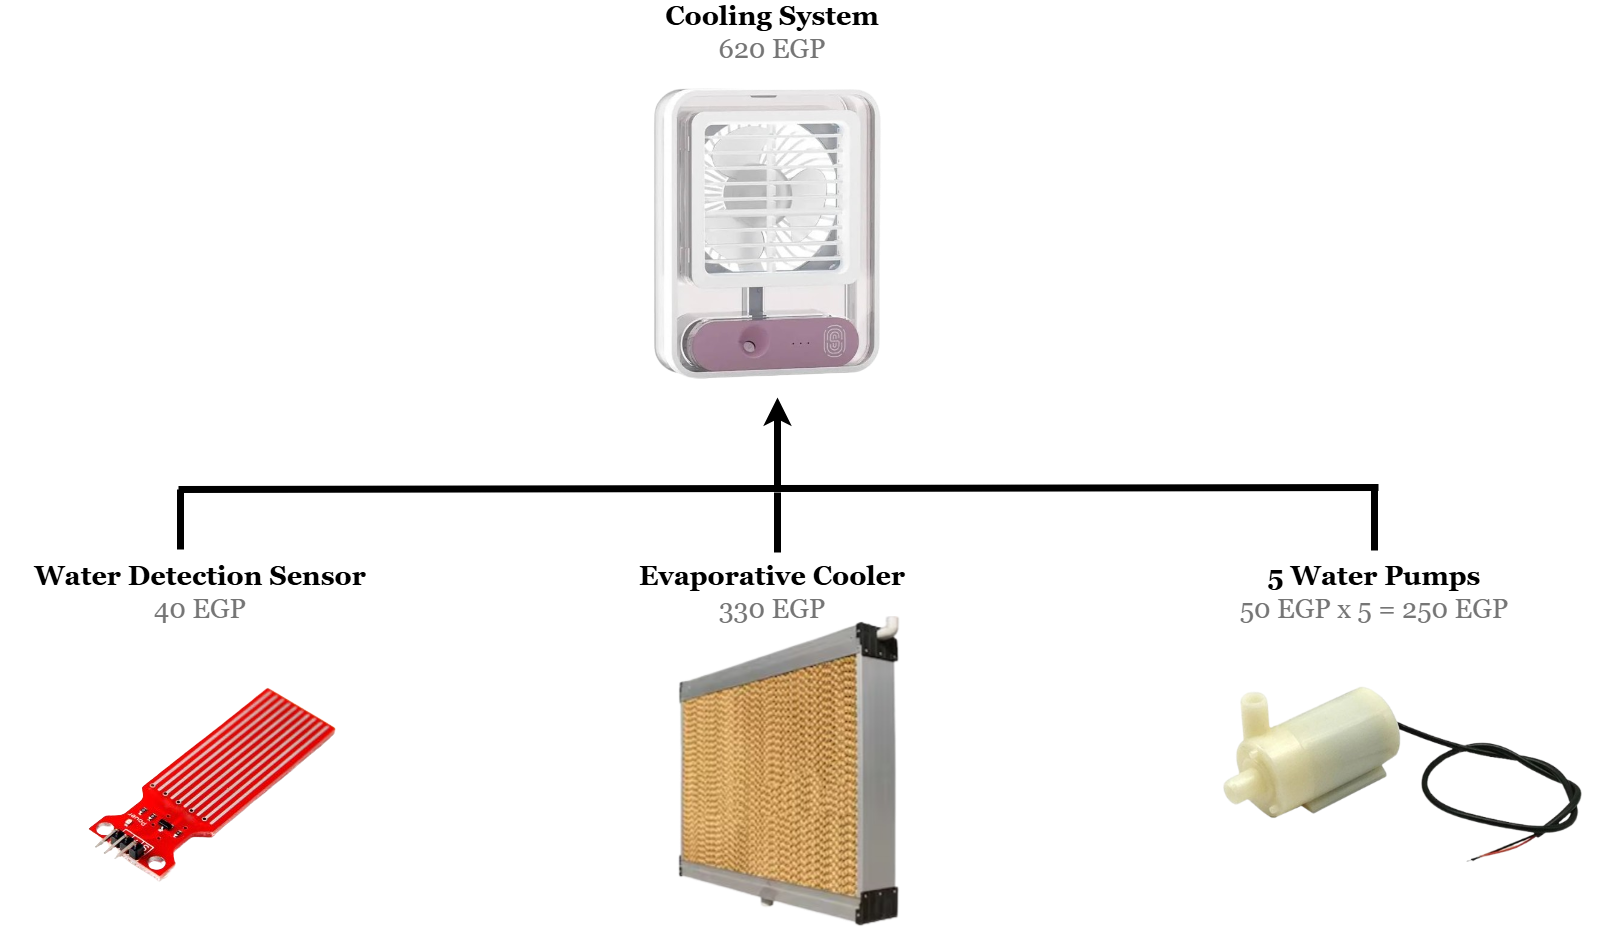
\includegraphics[width=0.7\textwidth]{Images/Components/Cooling System Cost.png}
		\caption{Cooling System Cost }
		\label{fig:COOLING_COST}
	\end{figure}
	\newpage
	\vspace{1 cm}
	\hspace{-0.65 cm}Ultimately, the actual cost of the system would not only be limited to one of each of these previously illustrated components, for they are merely compartmentalized segments of what the approximated overall production expense might be. The \textit{estimated} total cost for producing one fully- equipped smart beehive is roughly \textbf{25,210 EGP}. Be that as it may, the projected budget for minimum prototyping, a beehive comprising a single unit of each module, having  \textit{only one} frame, is estimated at \textbf{3,850 EGP}. While the prototyping build might fall short in meeting all the projects' features, it does offer a foundational build that would ease the testing and validation processes, while also reducing preliminary costs.
	\vspace{1.5 cm}
	\begin{figure}[H]
		\centering
		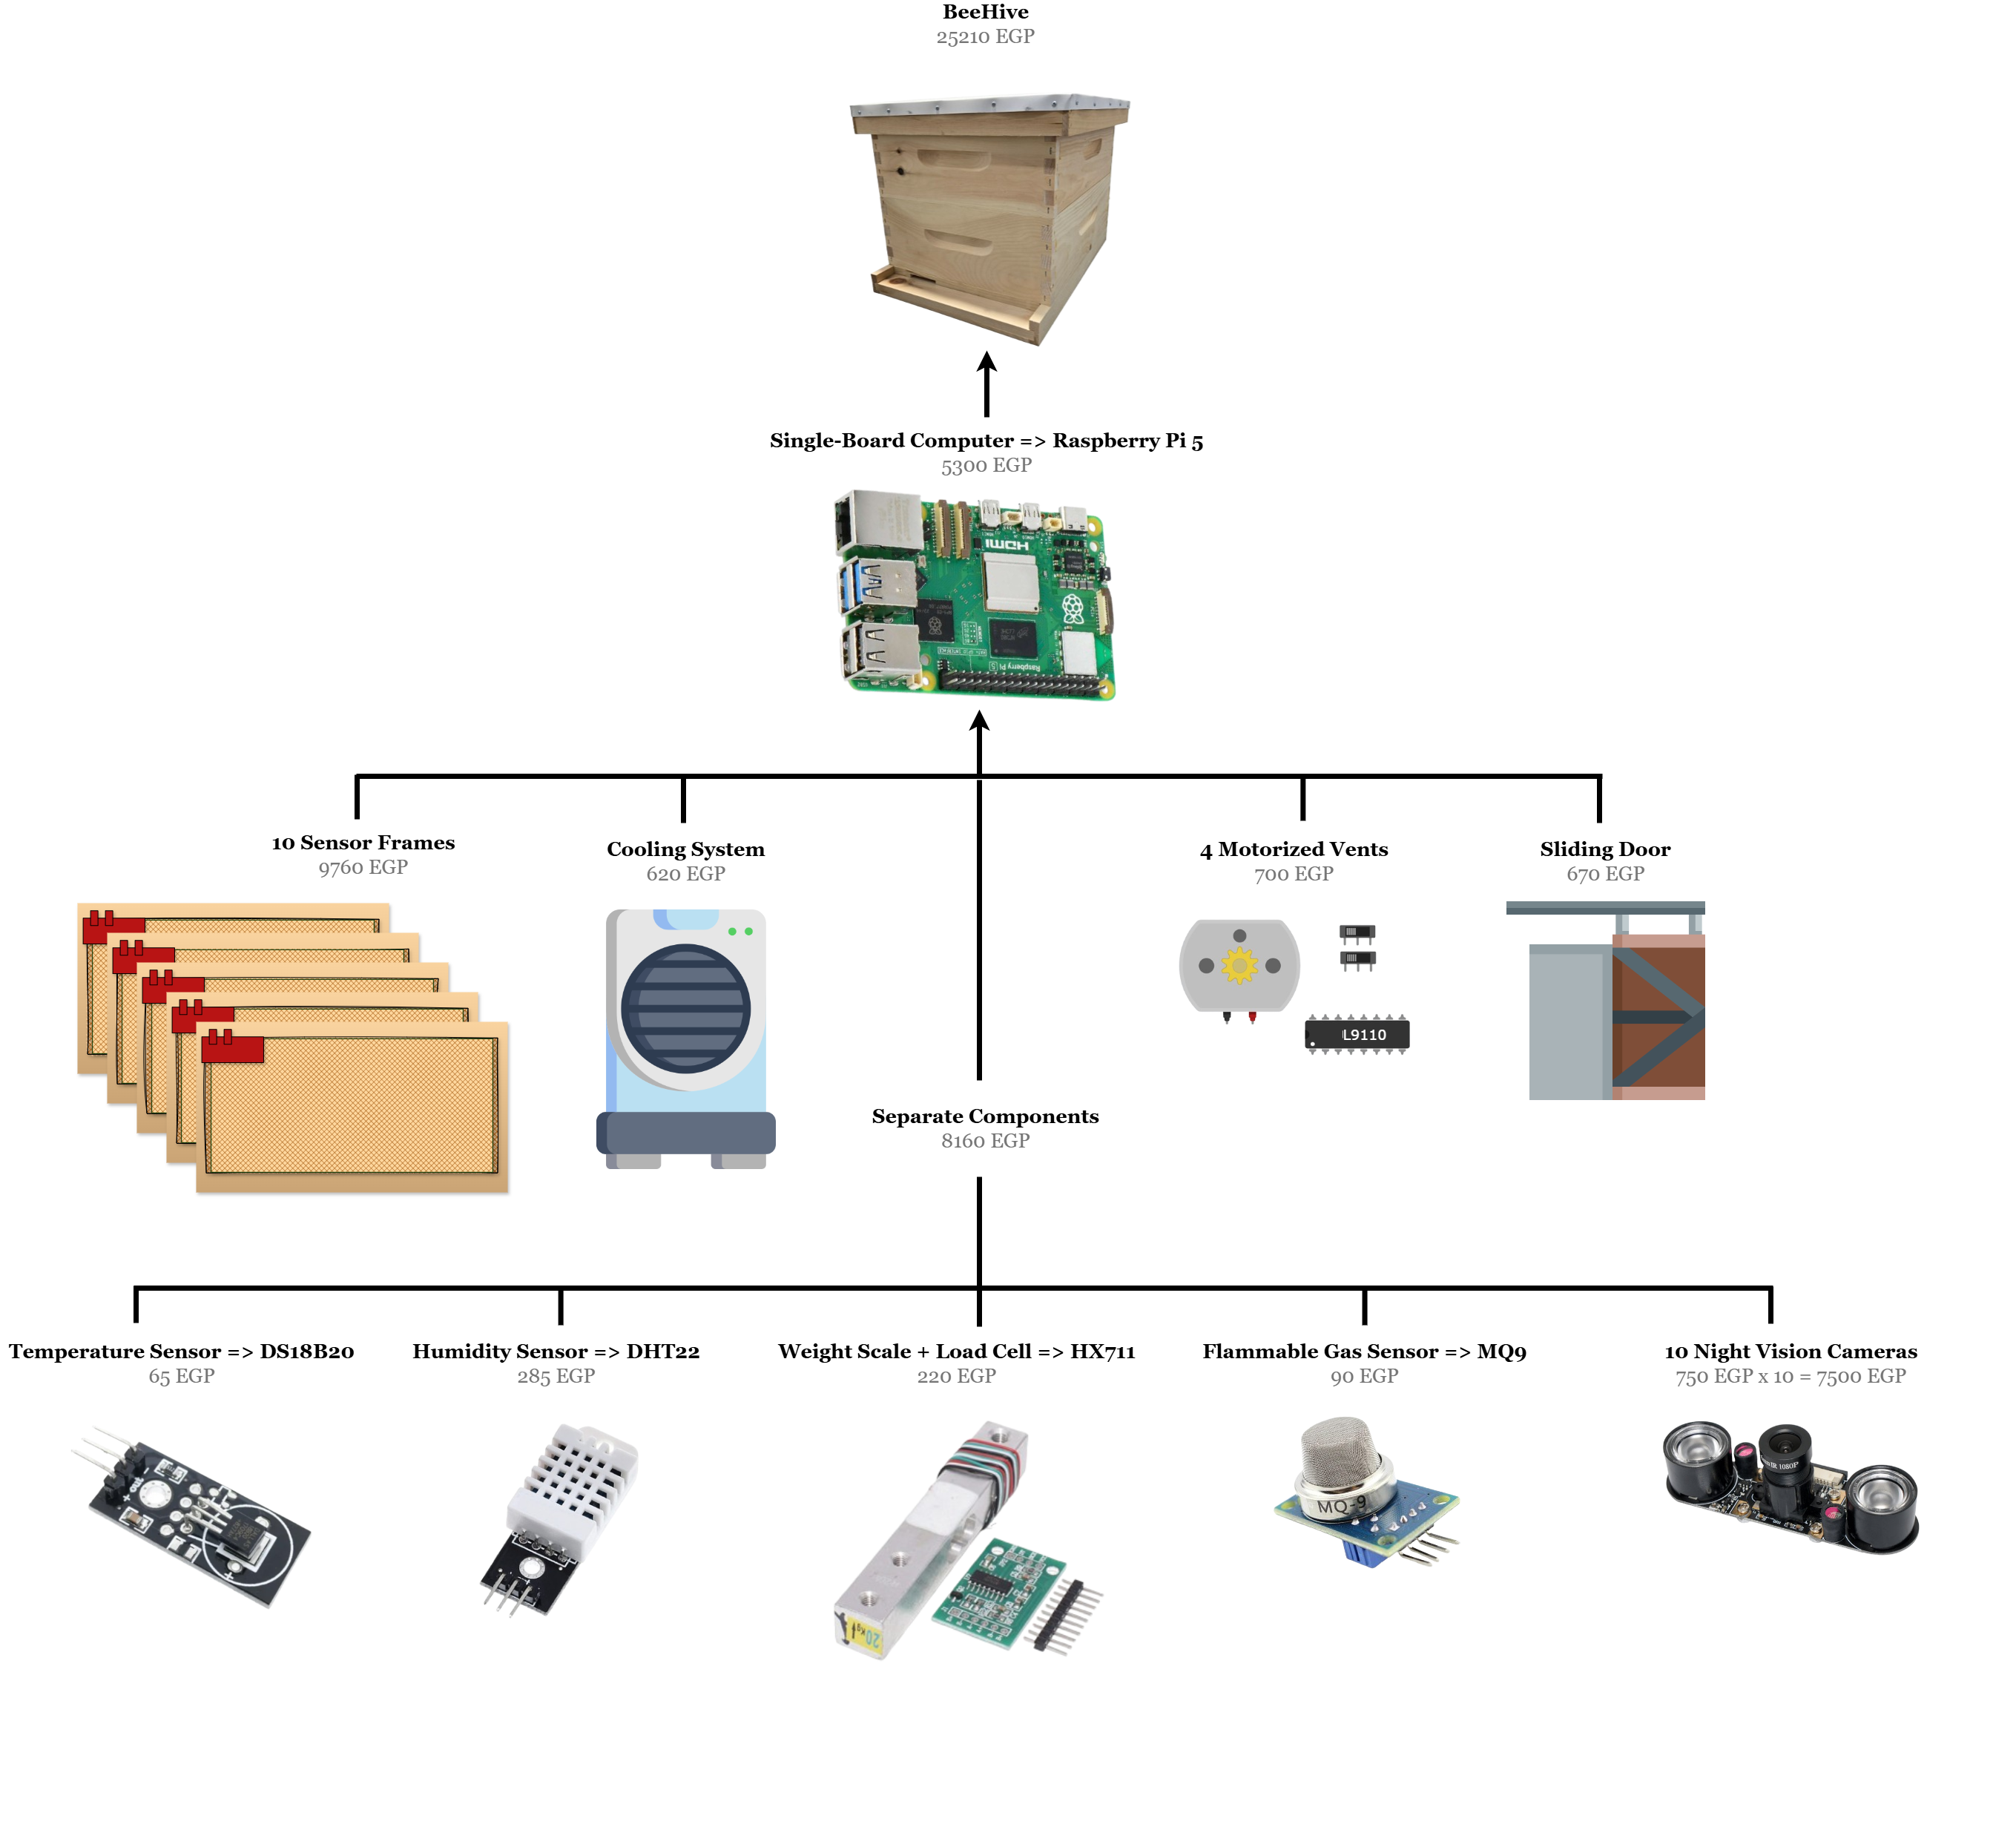
\includegraphics[width=\textwidth]{Images/Components/Total Cost.png}
		\caption{Total Cost }
		\label{fig:TOTAL_COST}
	\end{figure}
	
	
	\section{Supportive Documents}
	\subsection{Dataset}
	\subsubsection{Insect Classification}
	The Insect classification dataset incorporates images of bees, wasps, and other insects from multiple different datasets. In addition, noise that imitates the look of a picture taken by a night vision camera is applied to the images, due to the lack of an actual dataset with night vision photos of bees and other insects.
	\vspace{1 cm}
	\begin{figure}[H]
		\centering
		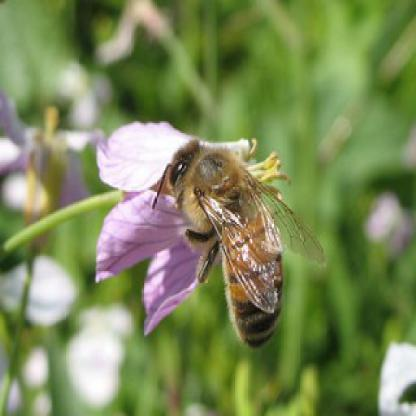
\includegraphics[width=0.5\linewidth]{Images/Sample/123 (1).jpg}
		\caption{A sample bee from the dataset}
		\label{fig:DATA_BEE}
	\end{figure}
	
	\begin{figure}[H]
		\centering
		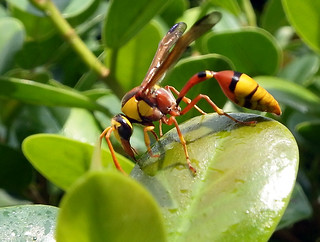
\includegraphics[width=0.5\linewidth]{Images/Sample/30319869311_5e35d23364_n.jpg}
		\caption{A sample Wasp from the dataset}
		\label{fig:DATA_WASP}
	\end{figure}
	\begin{figure}[H]
		\centering
		\begin{minipage}{0.45\textwidth}
			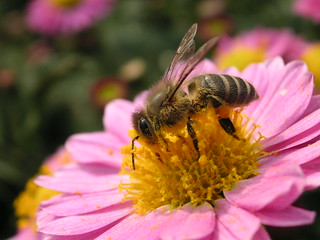
\includegraphics[width=\textwidth]{Images/Sample/1240800_e5f2b40032_n.jpg}
			\caption{A sample bee before night vision simulation}
			\label{fig:DATA_NORMAL}
		\end{minipage}
		\hfill
		\begin{minipage}{0.45\textwidth}
			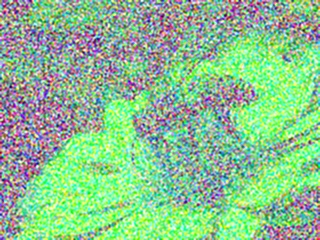
\includegraphics[width=\textwidth]{Images/Sample/1240800_e5f2b40032_n-nv.jpg}
			\caption{A sample bee after night vision simulation}
			\label{fig:DATA_NV}
		\end{minipage}
	\end{figure}
	
	
	\subsubsection{Capped and Uncapped Supers}
	This dataset contains images of honeycomb supers and each image is given a label, either capped or uncapped. Feeding this information to a model is crucial in implementing a honey-yield tracker, which would help beekeepers identify when honey, \textit{or wax}, are ready for collecting.
	
	\subsubsection{Buzzing Sounds}
	This dataset \cite{kaggle_to_bee_or_not_to_bee} includes audio clips of numerous beehives. Each audio clip has been meticulously labeled with timestamps for when there is an apparent buzzing sound presumably caused by a bee, or perhaps, at times, a potentially intruding wasp, and when there isn't. Having an acoustic model of sort would assist in asserting the presence of passing insects.
	
	
	\subsubsection{Sensor Readings}
	Readings of temperature and humidity will be collected from the hive using the sensors and then they will be used in tandem with a weather API to forecast the future values to decide whether to use counteractive measures or not. Furthermore, readings from the weight and vibration sensors will be collected. The weight data will be used for honey yield tracking, and used alongside the vibration data for anomaly detection. Furthermore, flammable gas sensor readings will be collected for safety alert thresholding.
	
	\subsection{Contacting Businesses}
	Through a meeting with the CEO of al badran, a company that owns honey farms in Egypt, Fouad Al-Badran shed light on many different aspects of bees, and beekeeping. Additionally, he so graciously agreed and offered to provide us with a suitable testing environment to with hold all of our work, which would be conducted at one of their apiaries.
	
	\printbibliography
\end{document}
